\documentclass[a4paper,11pt]{article}

\usepackage{amsmath, amssymb, amstext, amsfonts, mathrsfs}


% \sffamily %schrift ohne Serifen

\usepackage[T1]{fontenc} 
% schriftencodierung f�r umlaute, trennung
% f\"ur Uni
\usepackage[latin1]{inputenc}
\usepackage{selinput}
% \usepackage[utf8x]{inputenc} 
\usepackage{bibgerm} 
% german bibliography
\usepackage[german]{babel}
%wichtig f�r deutschen Content
\usepackage{ucs}
%erweiterte UTF-8 Unterst�tzung
\usepackage{wrapfig} 
% Paket zur Positionierung einbinden
\usepackage{multirow}
% zusammenfassen von Tabellenzellen
% \usepackage{subscript}
% zum tiefstellen
\usepackage{lscape}
\usepackage{pdflscape}
% zum drehen der Seite
% \usepackage[super]{natbib}
\usepackage[square,sort,comma,numbers]{natbib}
% Erstellung es Literaturverzeichnisses
\usepackage{url}
% Umbruch f�r URL
\usepackage{pst-3dplot}
% f�r tex Grafiken n�tig
\usepackage{pstricks}
\usepackage{listings}
% f�r das einf�gen von Quelltext
\definecolor{codegray}{rgb}{0.92,0.92,0.92}
\lstset{basicstyle=\fontsize{9}{11}\selectfont\ttfamily, breaklines=true, backgroundcolor=\color{codegray}, numbers=left, numberstyle=\tiny, tabsize=4, language=java, captionpos=b}
\definecolor{mymauve}{rgb}{0.58,0,0.82}
\definecolor{mygreen}{rgb}{0,0.6,0}
\lstset{
commentstyle=\color{mygreen},
keywordstyle=\color{mymauve},
language=Java,
stringstyle=\color{blue}
}


%Einstellungen f�r Quellcode
\usepackage[a4paper, left=3cm, right=2cm, top=2cm]{geometry}
% Formatierung R�nder
\usepackage[section]{placeins}
% f�r Floatbarriere
\usepackage{color}
\usepackage{colortbl}
%f�r die Verwendung von Farben

\clubpenalty = 10000 
\widowpenalty = 10000
\displaywidowpenalty = 10000
%Verhinderung von Hurenkindern und Schusterjungen
%10000 bedeutet die sie sollen kommplett vermieden werden

\title{Konzept und prototypische Implementierung eines �bergreifenden Dokumenten- und Medienmanagements als SOA-Anwendung}

\author{Sebastian Rieger}

\pagenumbering{arabic}
%Seitenzahlen(arabische Zahlen)

\setlength{\parindent}{0.25cm} 
%Absatzeinzug �ndern in Zoll
\setlength{\parskip}{0.25cm}
%Absatzabstand
% \linespread {1.5}
%Zeilenabstand

\usepackage{setspace}
\usepackage{hyperref}
%anklickbare Hyperlinks

%funktioniert nicht bei Fu�noten
\usepackage{graphicx}
\usepackage{graphics}
%f�r einbinden von Grafiken

\usepackage{framed}
%f�r Umrandung der Erkl�rung
\usepackage{acronym}
% f�r abk�rzungen
% \usepackage{PSTricks}
\usepackage{epstopdf}
% f�r eps bilder nutze pdflatex --shell-escape this.tex
\usepackage{amssymb}
% f�r mathematische Symbole

\usepackage{hyperref}
% klickbare links

% \usepackage{pdfpages}
\usepackage{rotating}
\usepackage{svg}
%%%%%%%%%%%%%%%%%%%%%%%%%%%%%%%%%%%%%%%%%%%%%%%%%%%%%%%%%%%%%%%%%%%%%%%%%%%%%%%%%%%%%%%%%%%%%%%%%%%%%
%% Angaben zur Arbeit
%%%%%%%%%%%%%%%%%%%%%%%%%%%%%%%%%%%%%%%%%%%%%%%%%%%%%%%%%%%%%%%%%%%%%%%%%%%%%%%

\newcommand{\Autor}{Sebastian Rieger}
\newcommand{\MatrikelNummer}{7406886}
\newcommand{\Kursbezeichnung}{TINF12B1}

\newcommand{\FirmenName}{Karlsruher Institut f�r Technologie (KIT)}
\newcommand{\FirmenStadt}{Karlsruhe}
\newcommand{\FirmenLogoDeckblatt}{{
\includegraphics[width=3cm]{Bilder/kitlogo}}}

% Falls es kein Firmenlogo gibt:
%  \newcommand{\FirmenLogoDeckblatt}{}

\newcommand{\BetreuerFirma}{Dipl. Inform. Thorsten Schlachter}
\newcommand{\BetreuerDHBW}{Dipl. Inform. (BA), MBA Christian Jordan}
\newcommand{\Titel}{Konzept und prototypische Implementierung eines �bergreifenden Dokumenten- und Medienmanagements}
\newcommand{\AbgabeDatum}{24.08.2015}

\newcommand{\Dauer}{12 Wochen}

% \newcommand{\Abschluss}{Bachelor of Engineering}
\newcommand{\Abschluss}{Bachelor of Science}

\newcommand{\Studiengang}{Angewandte Informatik}
% \newcommand{\Studiengang}{Angewandte Informatik}
\newcommand{\Was}{Bachelorarbeit}

%%%%%%%%%%%%%%%%%%%%%%%%%%%%%%%%%%%%%%%%%%%%%%%%%%%%%%%%%%%%%%%%%%%%%%%%%%%%%%%%%%%%%%%%%%%%%%%%%%%%% 
%steuervariableISO 23081
\usepackage{ifthen} %Package f�r if/else
\newboolean{bilder} %Deklaration
\setboolean{bilder}{true} %Zuweisung
% \setboolean{bilder}{false} %Zuweisung
%%%%%%%%%%%%%%%%%%%%%%%%%%%%%%%%%%%%%%%%%%%%%%%%%%%%%%%%%%%%%%%%%%%%%%%%%%%%%%%%%%%%%%%%%%%%%%%%%%%%%

\begin{document}

\begin{center}
\vspace*{-2cm}
\FirmenLogoDeckblatt\hfill
\includegraphics[width=4cm]{Bilder/dhbw-logo}\\[1cm]
{\Huge \Titel}\\[2cm]
{\Huge\scshape \Was}\\[2cm]
{\large f�r die Pr�fung zum}\\[0.5cm]
{\Large \Abschluss}\\[0.5cm]
{\large des Studienganges \Studiengang}\\[0.5cm]
{\large an der}\\[0.5cm]
{\large Dualen Hochschule Baden-W�rttemberg Karlsruhe}\\[0.5cm]
{\large von}\\[0.5cm]
{\large\bfseries \Autor}\\[1cm]
{\large Abgabedatum \AbgabeDatum}
\vfill
\end{center}
\begin{tabular}{l@{\hspace{1cm}}l}
Bearbeitungszeitraum             & \Dauer                       \\
Matrikelnummer                   & \MatrikelNummer              \\
Kurs                             & \Kursbezeichnung             \\
Ausbildungsfirma                 & \FirmenName                  \\
                                 & \FirmenStadt                 \\
Betreuer der Ausbildungsfirma    & \BetreuerFirma               \\
Gutachter der Studienakademie    & \BetreuerDHBW                \\
\end{tabular}

\newpage
%Seitenumbruch
%%%%%%%%%%%%%%%%%%%%%%%%%%%%%%%%%%%%%%%%%%%%%%%%%%%%%%%%%%%%%%%%%%%%%%%%%%%%%%
%% Descr:       Vorlage für Berichte der DHBW-Karlsruhe, Erklärung
%% Author:      Prof. Dr. Jürgen Vollmer, vollmer@dhbw-karlsruhe.de
%% $Id: erklaerung.tex,v 1.2 2010/07/22 13:30:27 vollmer Exp $
%%%%%%%%%%%%%%%%%%%%%%%%%%%%%%%%%%%%%%%%%%%%%%%%%%%%%%%%%%%%%%%%%%%%%%%%%%%%%%%

% In Bachelorarbeiten muss eine schriftliche Erklärung abgegeben werden. In allen anderen
% Arbeiten entf�llt diese. Hierin best�tigen die Studierenden, dass die Bachelorarbeit
% selbst�ndig verfasst und s�mtliche Quellen und Hilfsmittel angegeben sind. Diese Erkl�rung
% bildet das zweite Blatt der Arbeit. Der Text dieser Erkl�rung muss auf einer separaten Seite
% wie unten angegeben lauten.

\newpage
\thispagestyle{empty}
\begin{framed}
\begin{center}
\Large\bfseries Erkl\"arung
\end{center}

\noindent
Gem\"a\ss{}�16 (3) der "`Studien- und Pr\"ufungsordnung f\"ur den Studienbereich
Technik"' vom 1.11.2007.

\medskip
\noindent
Ich habe die vorliegende Arbeit selbstst\"andig verfasst und
keine anderen als die angegebenen Quellen und Hilfsmittel verwendet.

\vspace{3cm}
\noindent
\underline{\hspace{4cm}}\hfill\underline{\hspace{6cm}}\\
Ort~~~~~Datum\hfill Unterschrift\hspace{4cm}
\end{framed}

%%%%%%%%%%%%%%%%%%%%%%%%%%%%%%%%%%%%%%%%%%%%%%%%%%%%%%%%%%%%%%%%%%%%%%%%%%%%%%%
\endinput
%%%%%%%%%%%%%%%%%%%%%%%%%%%%%%%%%%%%%%%%%%%%%%%%%%%%%%%%%%%%%%%%%%%%%%%%%%%%%%%

\newpage
\begin{spacing}{0.9}

%Einf�gen Inhaltsverzeichnis
\tableofcontents



\end{spacing}

\newpage
\section{Abstract}
\newpage
\section{Einleitung} \label{Einfuehrung}
Beh\"orden und Firmen haben heute immer gr\"o\ss{}ere Datenbest\"ande zu verwalten, welche schon in elektronischen Systemen vorzufinden sind. Da diese Systeme historisch bedingt gewachsen sind, entstanden im laufe der Zeit immer mehr kleinere Insell\"osungen, welche ein \"ubergreifendes Verwalten und Nutzen von Daten erschwert oder gar ganz verhindert.

Das Ziel dieser Arbeit soll es daher sein, ein Konzept sowie eine prototypische Implementierung zu ertsellen, welche ein \"ubergreifendes und vereinheitlichtes arbeiten mit den Datenbest\"anden erm\"oglicht. Heutige \ac{DMS} Systeme decken eine vielzahl von Anwendungsgebieten ab, welche an die jeweiligen Problemstellungen wie Rechtsfragen oder fachliche Anforderungen angepasst sind oder angepasst werden k\"onnen.
Ein genaues Konzept mit Anforderungen, soll am Beispiel der \ac{LUBW} sowie der \ac{GAA} entstehen.
\cite{Dokumenten-Management}

Es sollen durch das Konzept auch bestehende Systeme weiter unterst\"utzt werden, wof\"ur hier eine Anbindungsm\"oglichkeit geschaffen werden soll. \"Uber eine serviceorientierte Anbinung sollen somit die verschiedensten Frontends wie Desktopanwendung, Web, Mobil usw. das neue Konzept nutzen k\"onnen. Welches \ac{ECM}-Tool f\"ur die Erstellung des Projekts am besten geeignet ist, muss analysiert werden, ergibt sich jedoch aus den zu verwaltenden Dokumenten.

F\"ur die Arbeit soll hierbei kein komplett neues \ac{DMS} mit Nutzer und Dokumentverwaltung entwickelt werden. Vielmehr soll evaluiert werden, welche Systeme es bereits auf dem Markt gibt, und wie sich diese f\"ur die anstehnde Aufgabe eignen, vor allem im Bezug auf die hierachische Gliederung der Metadaten, wie im Projekt vorgesehen ist. 

Als sogenannter \ac{PoC} soll im Verlauf dieser Arbeit ein bestehendes Fachsystem auf der Basis einer erarbeiteten Schnittstelle nachgebaut werden. Diese Frontend soll das derzeitige \ac{FADO}-System der \ac{LUBW} nachbilden.
\newpage
\section{Lastenheft} \label{Lastenheft}
An das Projekt, welches im Rahmen dieser Arbeit bearbeitet werden soll, gibt es viele Anforderungen. Um alle Anforderungen m\"oglichst strukturiert und \"Ubersichtlich darzustellen, wurde die Form eines Lastenhefts gew\"ahlt.

\subsection{Zielsetzung} \label{Zielsetzung}
Ziel ist es ein einheitliches \ac{ECM} System zu entwerfen, welches m\"oglichst alle Fachdokumente der \ac{LUBW} und der \ac{GAA} beinhaltet.
Hierbei sollen alle bestehenden und zuk\"unfitgen Systeme \"uber eine Schnittstelle mit dem \ac{DMS} kommunizieren.

\subsection{Produkteinsatz} \label{Produkteinsatz}
Bei dem zu entwickelnden System, handelt es sich um einen Prototyp f\"ur ein \ac{DMS}, welches gegebenenfalls von der \ac{LUBW} und der \ac{GAA} eingesetzt werden kann. Das zu entwickelnde Backend, soll alle Dokumente, welche schon heute auf den Websiten zu finden sind zusammenf\"uhren und diese in einer geeigneten Form ablegen.

\subsubsection{Zusammenspiel mit anderen Systemen} \label{Zusammenspiel mit anderen Systemen}
Das Backend soll nicht die heutigen Insell\"osungen f\"ur Dokumentverwaltung der \ac{LUBW} und der \ac{GAA} vereinen. Es sollen sowohl die bestehenden als auch zuk\"unfitge Systeme unterst\"utzt werden. Die jeweils ben\"otigten Daten, sollen hierf\"ur \"uber eine oder gegebenenfalls mehrere Schnittstellen erreichbar sein.

\subsection{Produktfunktionen} \label{Produktfunktionen}
\begin{minipage}{3cm}
/LF10/
\end{minipage}
\begin{minipage}{13cm}
Schon bestehende Dokumente sollen aus den alten Systemen \"ubernommen werden k\"onnen, ohne das ihre Metadaten verloren gehen oder ge\"andert werden. Dies bedeutet, dass das neue System den schon vorhandenen Datenbestand abbilden muss.\\
\end{minipage}
\begin{minipage}{3cm}
/LF20/
\end{minipage}
\begin{minipage}{13cm}
Die Metadaten der einzelnen Dokumente sollen fachlich und technisch gegliedert werden. Hierbei sollen gegebenenfalls Gruppierungen erstellt werden. Zum Beispiel sollen Longitude und Latitude zur Metadaten-Gruppe "`Geodata"' zusammengefasst werden.\\
\end{minipage}
\begin{minipage}{3cm}
/LF30/
\end{minipage}
\begin{minipage}{13cm}
Die Dokumente sollen ebenfalls nach den einzelnen Anwendungen und Fachbereichen gruppiert werden. Hier sollen die Anwendungen auch speziell ihre Dokumente nach Gruppenzugeh\"origkeit abfragen k\"onnen. Dies ist wichtig, da im \ac{FADO} nur die entsprechenden \ac{FADO}-Dokumente angezeigt werden sollen.\\
\end{minipage}
\begin{minipage}{3cm}
/LF40/
\end{minipage}
\begin{minipage}{13cm}
Eine Suche \"uber die Dokumente und ihre Metadaten soll grunds\"atzlich m\"oglich sein. Hier muss der Nutzer aber auch in der Lage sein die Suche weiter einzuschr\"anken oder nur nach bestimmten Metadaten suchen zu k\"onnen.\\
\end{minipage}
\begin{minipage}{3cm}
/LF50/
\end{minipage}
\begin{minipage}{13cm}
Die alten Systeme sollen durch das neue Backend keinerlei Einschr\"ankungen im Funktionsumfang unterworfen sein. Dies muss gegebenenfalls durch verschiedene Arten von Schnittstellen realisert werden.\\
\end{minipage}
\begin{minipage}{3cm}
/LF60/
\end{minipage}
\begin{minipage}{13cm}
F\"ur den Frontend-Prototyp, soll die Kernfunktionalit\"at einer Schnittstelle funktionsf\"ahig sein, anhand dessen der Prototyp evaluiert werden kann.\\
\end{minipage}

\subsection{Produktdaten} \label{Produktdaten}
\begin{minipage}{3cm}
/LD10/
\end{minipage}
\begin{minipage}{13cm}
Die entsprechenden Metadaten zu Dokumenten sollen durch das Backend verwaltet werden. Hierbei sollen nicht nur die manuell hinzugef\"ugten Metadaten beachtet werden, sondern auch die Metadaten, welche das Dateiformat liefert und solche die das Dokument enth\"alt.\\
\end{minipage}
\begin{minipage}{3cm}
/LD20/
\end{minipage}
\begin{minipage}{13cm}
Metadaten sollen nach M\"oglichkeit so zusammengefasst werden, das eine Oberklassenbildung und Vererbung von Metadaten m\"oglich ist. So soll zum Beispiel ein Standort alle Adressdaten zusammenfassen. Ein Standort wiederum kann in mehreren Dokumenten verwendet werden, wie zum Beispiel in Bildern oder in einem Forschungsbericht. Wiederum k\"onnte der Standort aber auch Betandteil der Unterklasse Gericht sein und somit den Standort des Gerichts abbilden.\\
\end{minipage}
\begin{minipage}{3cm}
/LD30/
\end{minipage}
\begin{minipage}{13cm}
Metadaten sollen \"ahnlich wie objektorientierte Klassen in Programmiersprachen agieren. So wird ein Autor "`Max Mustermann"' nur einmal angelegt. Er kann jedoch in mehreren Dokumenten auftauchen. Sucht ein Nutzer nach "`Max Mustermann"', so werden ihm alle Eintr\"age zu diesem angezeigt. Vergleichen kann mal diese Art von Abbildung auch mit einer relationalen Abbildung wie sie in Datenbanken zu finden ist.\\
\end{minipage}
\begin{minipage}{3cm}
/LD40/
\end{minipage}
\begin{minipage}{13cm}
F\"ur die Gliederung der Metdaten sollen auch schon bestehende Standards betrachtet und gegebenenfalls umgesetzt werden.
Im Verlauf der Arbeit muss evaluiert werden, welche Standards es f\"ur Metadaten gibt und wie sie im Projekt umgesetzt werden m\"ussen und k\"onnen.
\cite{Wiki_Dublin_Core} \cite{Wiki_ISO_19115} \cite{Wiki_Exif} \cite{Wiki_Inspire}\\
\end{minipage}


\subsection{Produktleistungen} \label{Produktleistungen}
\begin{minipage}{3cm}
/LL10/
\end{minipage}
\begin{minipage}{13cm}
Das Backend soll f\"ur Dokumente, welche in verschiedenen Versionen vorliegen eine Art Versionsverwaltung bieten, so das auch \"altere Versionen zug\"anglich sind. Dies zum Beispiel bei Gesetzestexten wichtig, da hier immer die zum Vorfall aktuelle Version betrachtet werden muss.\\
\end{minipage}
\begin{minipage}{3cm}
/LL20/
\end{minipage}
\begin{minipage}{13cm}
Die Dokumente sollen \"uber verschiedene Schnittstellen wie zum Beispiel eine \ac{REST}-Schnittstelle abgerufen werden k\"onnen. Der Einsatz von \ac{API}s ist je nach \ac{ECM}-Tool gegebenenfalls auch m\"oglich, jedoch ist eine solche Ums\"atzung nicht Teil der Arbeit. \cite{Wiki_REST}\\
\end{minipage}
\begin{minipage}{3cm}
/LL30/
\end{minipage}
\begin{minipage}{13cm}
Eine Suche \"uber Metadaten muss realisert werden. Hierbei soll dem Nutzer zum einen eine grobe aber auch zum anderen eine verfeinerte eingeschr\"ankte Suche nach bestimmten Metadaten geboten werden.\\
\end{minipage}
\newpage
\section{Stand der Technik / existierende Konzepte} \label{Stand der Technik}
Im folgenden Kapiel werden die einzelnen Fachsysteme, der \ac{LUBW} und deren Datenbest\"ande genauer analysiert. Zus\"atzlich wird ein Blick auf das Literaturarchiv der \ac{ICT-ENSURE} gerichtet, um ein m\"oglichst \"ubergreifendes Metadatenmodell erstellen zu k\"onnen. 

Welche Metdaten die einzelnen Dokumentenbest\"ande der Fachsysteme genau enthalten ist im Anhang \ref{Metadaten der LUBW Fachsysteme} genau aufgelistet. Hierbei wird unterschieden, ob es sich um Metadaten oder relationen handelt. Daf\"ur wurden alle Metadaten aus den Systemen extrahiert.


Die Metadaten der in diesem Kapitel untersuchten Systeme werden anschlie\ss{}end im Kapitel \ref{Erstellung eines Datenkonzepts} zu einem \"ubergreifenden Metadatenmodell vereint, welches die sp\"atere Grundlage f\"ur ein \ac{ECM}-Tool sein soll.

% Die einzelnen Fachsysteme der \ac{LUBW} sind f\"ur unterschieliche Einsatzzwecke entwickelt wurden, welche nun genauer anlaysiert werden.
% Ebenso wird das Literaturarchiv der \ac{ICT-ENSURE} untersucht, um ein \"ubergreifendes Datenmodell zu erstellen.

\subsection{FADO und Untergruppen} \label{FADO}
Das \ac{FADO}-System der \ac{LUBW} erlaubt es den Nutzern nach verschiedenen Texten aus unterschielichen Themenrichtungen zu suchen und diese herunterzuladen. Hierbei stehen die Dokumente, zum Teil wahlweise, im PDF- oder HTML-Format bereit.

Die einzelnen Ver\"offentlichungen k\"onnen nach verschiedenen Kriterien durchsucht werden, wobei der Bestand an Dokumenten, von der \ac{LUBW} fortlaufend erweitert wird.
\cite{LUBW_FADO}

Im \ac{FADO}-System sind die Dokumente in die sechs Kategorien Altlasten, Boden, Natur und Landschaft, Umweltbeobachtung, Umweltforschung und Umweltinformationssysteme gegliedert. Hierbei ist zu beachten, dass ein Dokument nicht nur einem Themengebiet zugeordent werden kann, sondern durchaus unter mehreren Gebieten zu finden ist. Solche Dokumente sind im \ac{FADO} jedoch nur einmal abgespeichert und werden \"uber Relationen den verschiedenen Kategorien zugeordent.

Die einzelnen Kategorien sind wiederum mit Untergruppen versehen, welche die Zugeh\"origkeit der Dokumente konkretisieren.

Da im Verlauf der Arbeit nicht alle Gruppen in ein neues System \"uberf\"uhrt werden k\"onnen, wird sich auf die Dokumentklassen Berichte, Urteile und Forschungsvorhaben beschr\"ankt, welche in der Kategorie Natur und Landschaft, in der Kategorie Boden beziehungsweise in der Kategorie Umweltforschung zu finden sind.

Forschungsvorhaben wiederum sind Berichte, welche sich in eine Skizze, einen Zwischen- und einen Abschlussbericht aufteilen. Hierbei geh\"oren die drei Teile zu jeweils einem Forschungsvorhaben. \cite{LUBW_FADO}

\subsection{Das Document Retrieval System} \label{DRS}
Das \ac{DRS} der \ac{LUBW} ist eine Art Suchmaschine, die es erm\"oglicht verschiedene Rechtsvorschriften, Regelungen, Fachberichte und Erl\"asse zu suchen. Abfragen im \ac{DRS} k\"onnen auf drei Arten erfolgen. Es gibt die "`Standardsuche"', welche es erlaubt nach Inhalt oder Metadaten der Dokumente zu suchen. Die "`Titelsuche"' erlaubt es, wie der Name schon sagt nach Titeln oder gegebenenfalls nach Normtiteln der Dokumente zu schauen. Als dritte M\"oglichkeit bietet das \ac{DRS} eine "`Geziehlte Suche"' an, die es erm\"oglicht Suchkriterien genau anzugeben und diese auch einzuschr\"anken.
\cite{DRS}

Zu beachten ist, dass das \ac{DRS} eine eigenst\"andiges Plattform ist, welche einen eigenen Dokumentenbestand vorh\"alt.

In Abbildung \ref{Suchmaske DRS} ist die Suchmaske der "`Geziehlten Suche"' vom \ac{DRS} zu sehen. Es werden in der Maske alle M\"oglichkeiten aufgef\"uhrt, nach denen gesucht werden kann, was alle vorhandenen Metadaten mit einschlie\ss{}t. Die meisten Metadaten, sind durch Auswahllisten beschr\"ankt und andere k\"onnen vom Nutzer frei mit Begrifflichkeiten gef\"ullt werden.

Zu sehen ist in den Feldern Fassung und \"Anderung, dass eine Art Verwaltung von \"alteren Versionen vorgenommen wird. Diese Versionierung ist notwendig, da alte Gesetzestexte f\"ur in der Vergangenheit liegende F\"alle aufbewahrt werden m\"ussen.

\begin{figure}[!ht]
\centering
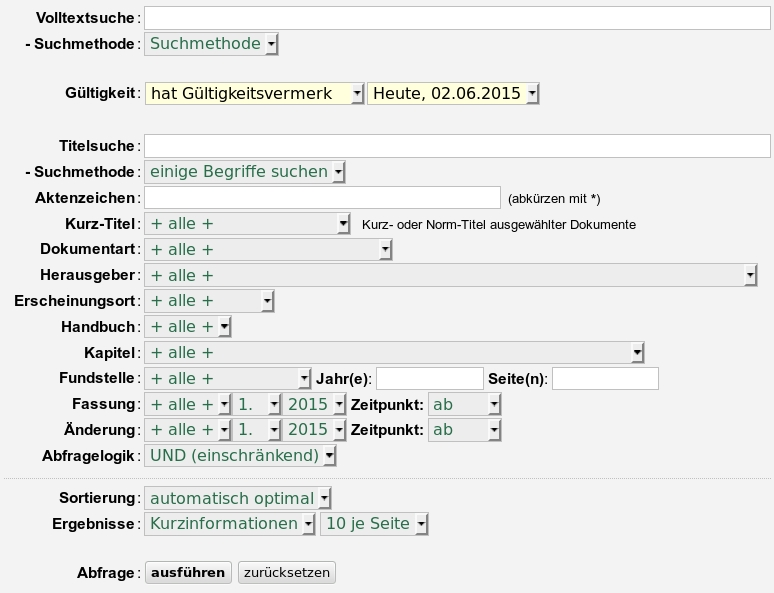
\includegraphics[width=15cm]{Bilder/Suchmaske_DRS.jpg}
\caption{Suchmaske des \ac{DRS}}
\label{Suchmaske DRS}
\centering
\end{figure}

\subsection{Naturschutz-Bildarchiv} \label{Bilddatenbank}
Im Naturschutz-Bildarchiv der \ac{LUBW} finden sich viele Bilder zu verschiedenen Themengebieten, so zum Beispiel auch zu den Gebieten Biotoptyp, Lebensraumtyp, Naturschutzgebiet und einige mehr.
\cite{Naturschutz-Bildarchiv}

Diese Themenkomplexe k\"onnen wiederum nach Stichworten durchsucht werden, wie zum Beispiel "`Aurorafalter"', was im Themengebiet "`Pflanzen- und Tierart"' Bilder von entsprechenden "`Faltern"' liefert. Auch das Bildarchiv ist ein eigenst\"andiges System, welches seinen eigenen Dokumentenbestand besitzt.

\subsection{Literaturarchiv der ICT-ENSURE}
Im Literaturarchiv der \ac{ICT-ENSURE} sind verschiedene Dokumente zu verschiedenen Themengebieten zu finden. Die \ac{ICT-ENSURE} ist ein EU-Projekt, welches es sich zur Aufgabe gemacht hat die Zusammenarbeit von Forschung und Wissenschaft in Europa zu st\"arken.

\ac{ICT-ENSURE} enth\"alt wie schon erw\"ahnt viele verschiedene Dokumente aus dem Breich Forschung und erlaubt eine Volltextsuche innerhalb dieser Dokumente. Zus\"atzlich sind die einzelnen Dokumente nach verschiedenen Fachrichtungen beziehungsweise Konferenzen gegliedert.
\cite{ICT-ENSURE_Bericht}

Alle Dokumente der \ac{ICT-ENSURE} sind B\"ucher, und so erfolgt auch ihre Speicherung.
Zu jeder Konferenz gibt es ein Buch, welches in Kapitel unterteilt ist. Diese Kapitel wiederum sind in Unterkapitel geteilt, welche den einzelnen Vortr\"agen entsprechen.

Eine genaue Auflistrung der Metadaten ist im Anhang \ref{Metadaten der ICT-ENSURE} zu finden.

\newpage
\section{Analyse von Metadatenstandards} \label{Analyse Datenbestaende}
Nach dem nun die Portale \ac{DRS}, Naturschutz-Bildarchiv und \ac{FADO}, der \ac{LUBW} und das Literaturarchiv der \ac{ICT-ENSURE} im Kapitel \ref{Stand der Technik} genauer betrachtet und die Verwaltungsstrukturen aufgezeigt wurden, betrachtet dieses Kapitel nun Standards f\"ur Metadaten. Hierbei wird unterschieden, ob es sich um fachliche oder technische Metadaten handelt.

\subsection{Fachlich}
Fachliche Metadaten sind Daten, welche den Inhalt einer Datei oder eines Dokuments genauer beschreiben und dem Anwender dabei helfen f\"ur ihn relevante Dateien zu identifizieren. Solche Metadaten sind immer fachspezifisch und unabh\"angig von den technischen Eigenschaften einer Datei.
\cite{Fachliche_Metadaten_Wissensportal_BI} \cite{Fachliche_Metadaten_msg} \cite{DHW_Wiki_Metadaten} \cite{Multimedia_retrieval}

Die Dokumente der Fachsysteme der \ac{LUBW}, sowie der \ac{ICT-ENSURE} enthalten alle fachliche Metadaten. Eine genaue Aufstellung aller fachlichen Metadaten der in dieser Arbeit untersuchten Dokumente ist im Anhang \ref{Metadaten der LUBW Fachsysteme} zu finden.

\subsection{Fachliche Metadaten-Standards} \label{Fachliche Metadaten-Standards}
F\"ur die Erstellung eines Datenkonzepts wie es im Kapitel \ref{Erstellung eines Datenkonzepts} geschieht, ist es aber nicht nur notwendig die vorhandenen Metadaten zu betrachten. Auch Standards f\"ur fachliche Metadaten sollen in diesem Umfeld untersucht werden.

Da fachliche Metadaten meist anwendungs- beziehungsweise dokumentbezogen sind, gibt es nicht sehr viele Standards, welche sich im Umfeld der \ac{LUBW} beziehungsweise der \ac{ICT-ENSURE} einsetzen lassen.

\subsubsection{Darwin Core}\label{Darwin Core}
Darwin Core beschreibt eine Zusammenfassung von Metadaten, welche f\"ur biologische Zwecke eingesetzt werden k\"onnen. So ist es zum Beispiel m\"oglich, Angaben zum Organismus oder zum Lebensraum zu machen. 

Hierf\"ur verwendet Darwin Core bis zu 172 Tags, welche jedoch nicht zwingend verwendet werden m\"ussen. Zus\"atzlich enth\"alt der Standard auch die Tags von Dublin Core (siehe Abschnitt \ref{Dublin Core}) um das Dokument grundlegend zu beschreiben.
\cite{Darwin_Core} \cite{Wiki_Darwin_Core}

Ii Listing \ref{Darwin Core Beispiel in XML}\footnote{\url{http://rs.tdwg.org/dwc/terms/guides/xml/index.htm}} ist einmal ein Beispiel f\"ur den Darwin Core-Standard  mit XML dargestellt. Es ist zu sehen, das ein "`SimpleDarwinRecord"' verwendet wird, welcher nicht alle 172 Tags beinhaltet. 

Es ist auch zu erkennen, dass die Dublin Core-Tags inbegriffen sind (beginnend mit "`dcterms"'). Die eigentliche Tags des Darwin-Standards beginnen mit "`dwc"'.
\lstinputlisting[caption=Darwin Core-Beispiel in XML, label=Darwin Core Beispiel in XML]{Code/Darwin_Core.xml}

\subsubsection{INSPIRE} \label{INSPIRE}
\ac{INSPIRE} ist ein Standard f\"ur Metadaten, welcher von der \ac{EU} nach der Richtlinie "`2007/2/EG"' vom 14. M�rz 2007 erlassen wurde. \ac{INSPIRE} enth\"alt Metadaten, welche f\"ur Geo-Referenzen benutzt werden m\"ussen, denn nach der eben genannten \ac{EU}-Richtlinie m\"ussen alle vom Land ver\"offentlichten digitalen Dateien mit Geo-Referenzen versehen werden.

\ac{INSPIRE} stellt 25 Meta-Tags zur Verf\"ugung, mit dessen Hilfe die \ac{EU}-Richtlinie zur Bekanntmachung von Geo-Referenzen eingehalten wird.
Au\ss{}erdem enth\"alt der \ac{INSPIRE}-Standard die notwendigen Tags der DIN EN ISO 19115 (siehe Abschnitt \ref{ISO 19115}), wodurch dieser gleichzeitig nach dieser Norm ISO-konform wird. 
\cite{INSPIRE_Richtlinie}

Von den 25 Meta-Tags m\"ussen 12 Tags zwingend angegeben werden, um die Richtlinie zu erf\"ullen. Die Meta-Tags von \ac{INSPIRE} sind zum Teil untergliedert, was bedeutet, dass eine Vielzahl mehr an Information in diesen Standard enthalten sein k\"onnen.

Aus \"Ubersichlichkeitsgr\"unden wird an dieser Stelle kein Beispiel Listing erfolgen, da das XML-Format von \ac{INSPIRE} sehr ausf\"uhrlich und gro\ss{} ist. Es wird jedoch an dieser Stelle auf den Editor f\"ur \ac{INSPIRE}-Metadaten der Europ\"aischen Kommission verwiesen, mit dessen Hilfe schnell und einfach XML-Dokumente mit \ac{INSPIRE}-Metadaten erzeugt werden k\"onnen\footnote{\url{http://inspire-geoportal.ec.europa.eu/editor/}}.
\cite{INSPIRE_Geoportal} \cite{Wiki_Inspire} 

\subsubsection{DIN EN ISO 19115} \label{ISO 19115}
Die DIN EN ISO 19115 ist eine Norm, welche 2005 spezifiziert wurde. Sie enth\"alt Metadaten f\"ur die Bescheibung von Geo-Information. Mit \"uber 400 m\"oglichen Tags ist sie eine der detailliertesten Beschreibungsstandards f\"ur Geo-Daten. 

Von den \"uber 400 Tags sind f\"ur eine Verwendung der Norm nur ca. 22 Tags erforderlich. Alle anderen Tags sind optional.
\cite{ISO_19115_Doku} \cite{Wiki_ISO_19115}

Wird der \ac{INSPIRE}-Standard verwendet (siehe Abschnitt \ref{INSPIRE}), so ist automatisch auch die ISO 19115 erf\"ullt, da diese Bestandteil  von \ac{INSPIRE} ist.
\cite{INSPIRE_Richtlinie}

\subsubsection{ONIX}
Der \ac{ONIX}-Standard ist international bekannt und f\"ur den elektronischen Austausch von Buchinformationen geschaffen worden.

\ac{ONIX} kann gem\"a\ss{} der Lizenz frei verwendet werden und ist zur Beschreibung von traditionellen B\"uchern und E-Books vorgesehen.
Der Standard enth\"alt sehr viele Tags, mit dessen Hilfe ein Buch beschrieben werden kann. So k\"onnen zum Beispiel Angaben zum Verleger und zur ISBN gemacht werden. \cite{ONIX} \cite{Wiki_ONIX}

Nachteilig ist, dass das Format sehr viel auf Abk\"urzungen setzt, was eine Menschenlesbarkeit  erschwert oder gar verhindert.

Ein kleines Beispiel zum \ac{ONIX}-Format ist im Listing \ref{ONIX Beispiel in XML} zu finden. Hier wird kurz beschrieben das es sich um einen Download handelt, welcher im Epub-Format vorhanden und lesbar ist. Ohne die Erkl\"arungen am Ende der Zeile w\"aren die Informationen nicht ohne weitere Hilfe lesbar. 

\lstinputlisting[caption=ONIX-Beispiel in XML, label=ONIX Beispiel in XML]{Code/ONIX.xml} \cite{ONIX_Example}


\subsection{Technisch}
Technische Metadaten sind Daten, die den internen Dateiaufbau und dessen Inhalt beschreiben. Sie betreffen den Anwender nur sekund\"ar und sind eher wichtig f\"ur die richtige Speicherung und f\"ur Administratoren. Technische Metadaten sind unabh\"angig von dem fachlichen Inhalt eines Dokuments und beschreiben zum Beispiel dessen Datenformat, das Erstellungsdatum oder die Nutzerrechte genauer.
\cite{Fachliche_Metadaten_Wissensportal_BI} \cite{Fachliche_Metadaten_msg} \cite{DHW_Wiki_Metadaten} \cite{Multimedia_retrieval}

In den Systemen der \ac{LUBW} und der \ac{ICT-ENSURE} werden keine technischen Metadaten angezeigt, weshalb diese an der Stelle nicht betrachtet werden.
Technische Metadaten sind vor allem bei physikalischen Daten wichtig. Da die Systeme nur intern mit diesen Daten arbeitenm werden sie dem Nutzer nicht angezeigt. In einem \ac{ECM}-System spielen sie jedoch eine wichtige Rolle und werden im sp\"ateren Verlauf der Arbeit genauer betrachtet. 

Ref?????

\subsection{Technische Metadaten-Standards}
Wie schon bei den fachlichen Metadaten (siehe Abschnitt \ref{Fachliche Metadaten-Standards}) gibt es auch f\"ur technische Metadaten Standards, welche versuchen, die Beschreibung von Dokumenten zu vereinheitlichen. In den folgenden Abschnitten werden nun einige Standards f\"ur technische Metadaten vorgestellt und genauer beschrieben.

\subsubsection{Dublin Core} \label{Dublin Core}
Dublin Core ist ein Standard, welcher ein Dokument grundlegend beschreibt. Von der \ac{DCMI}, welche den Standard beschlossen, hat werden 15 Kernfelder zur Verwendung, die so genannten "`core elements"', empfohlen. Es gibt jedoch weitere Felder, welche zus\"atzliche Informationen enthalten k\"onnen.
\cite{Wiki_Dublin_Core} \cite{Dublin_Core} \cite{Multimedia_retrieval}

Der Standard sollte heute Bestandteil jeder Website sein, da viele Suchmaschinen wie zum Beispiel Google nach Dublin Core-Metadaten suchen und Ergebnisse zum Beispiel anhand dieser Filtern. Ist also eine \ac{SEO} angedacht beziehungsweise wie in \ac{FADO} umgesetzt, sollten diese Metadaten vorhanden sein.
\cite{Dublin_Core_und_SEO}

Ein Beispiel f\"ur Dublin Core ist im Listing \ref{Dublin Core Beispiel in HTML}\footnote{\url{http://de.wikipedia.org/wiki/Dublin_Core}} zu finden. Hier wird der Standard im HTML-Format verwendet. Es wird zum einen auf das offizelle Schema verlinkt, zum anderen werden die einzelnen Metadaten dargestellt, welche in den Meta-Tags zu finden sind, und mit dem Namen "`DC."' beginnen, um zu verdeutlichen, dass es sich hier um Dublin Core handelt.

\lstinputlisting[caption=Dublin Core-Beispiel in HTML, label=Dublin Core Beispiel in HTML]{Code/Dublin_Core.html}

\subsubsection{Exif} \label{Exif}
Das Exif-Metadatenformat ist ein Standard f\"ur die Beschreibung von Bildern. In der heutigen Zeit verf\"ugen nahezu alle digitalen Kameras \"uber dieses Format und speichern bei der Aufnahme eines Bildes verschiedene Parameter im \ac{Exif} ab. 
\cite{Wiki_Exif}

Mit \"uber 50 Tags kann ein Bild mit Hilfe von \ac{Exif} sehr detailiert beschrieben werden. Es gibt unter anderem Tags f\"ur die Belichtungszeit, die Blende und den Farbraum. Aber auch Koordinaten, an dem das Bild aufgenommen wurde, k\"onnen vorhanden sein.
\cite{Wiki_Exif} \cite{Exif_Spezifikation}

Eine genaue Auflistung aller Tags und deren Inhalt ist in der Spezifikation "`Exchangeable Image File Format for digital still cameras"'\footnote{\url{http://www.jeita.or.jp/japanese/standard/book/CP-3451C_E/\#page=1}} zum Format zu finden.

\subsubsection{RDF} \label{Rdf}
Das \ac{RDF} ist im eigentlichen Sinn keine Beschreibung von standardisierten Metadaten. Vielmehr ist es ein \"ubergeordneter Standard, der beschreibt, wie Metadaten beschrieben werden k\"onnen.
\cite{Wiki_RDF}

Hierf\"ur wird eine Satzstruktur verwendet, welche jeweils aus Subjekt, Pr\"adikat und Objekt besteht. Am folgenden Beispiel in Abbildung \ref{RDF Struktur} wird verdeutlicht, was genau mit einer Satzstruktur gemeint ist. \cite{Multimedia_retrieval}

\begin{figure}[!ht]
\centering
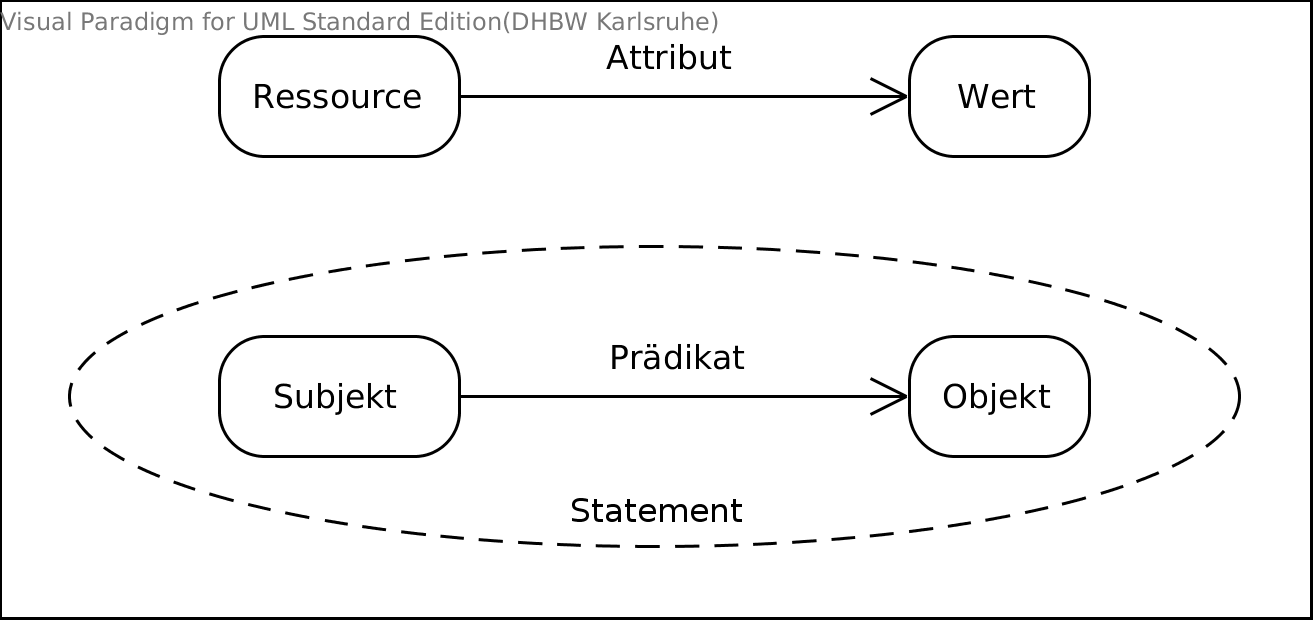
\includegraphics[width=8cm]{Bilder/RDF.png}
\caption{Struktur von \ac{RDF}}
\label{RDF Struktur}
\centering
\end{figure}

Mit Hilfe von \ac{RDF} kann also ausgesagt werden, dass eine Website "`www.beispiel.com"' ein Erstellungsdatum am 15.06.2015 hat.
Somit ergibt sich die Aufteilung:
\begin{itemize}
 \item Subjekt: www.beispiel.com
 \item Pr\"adikat: hat Erstellungsdatum
 \item Objekt: 15.06.2015
\end{itemize}

In XML w\"urde dieses Beispiel wie im Listing \ref{RDF in XML} aussehen.
\cite{Multimedia_retrieval}

\lstinputlisting[caption=RDF-Beispiel in XML, label=RDF in XML]{Code/RDF.xml}

\subsubsection{ANSI/NISO Z39.87-2006 (R2011)} \label{R2011}
Das ANSI/NISO Z39.87-2006 ist ein amerikanisches nationales Format, welches Bilddateien beschreibt. Es ist \"ahnlich aufgebaut wie \ac{Exif} und enth\"alt grundlegend die selben M\"oglichkeiten wie das im Abschnitt \ref{Exif} vorgestellte \ac{Exif}. \cite{NISO_Standard}

Da sich die Arbeit jedoch mit europ\"aischen Projekten und Organisationen besch\"aftigt, wird auf dieses Format hier nicht weiter eingegangen.
\newpage
\section{Erstellung eines Datenkonzepts} \label{Erstellung eines Datenkonzepts}
Im nun folgenden Kapitel werden die zuvor in den Kapiteln \ref{Stand der Technik} und \ref{Analyse Datenbestaende} beschriebenen Metadaten der einzelnen Systeme zu einen umfassenden Datenkonzept zusammengefasst. Dieses Konzept bildet die Grundlage zur Speicherung in einem \ac{DMS}.

Zuerst wird das Metadatenmodell m\"oglichst weit "`normalisiert"' und aufgebrochen. Dies ist wichtig um Gemeinsamkeiten bei dem Metadaten zu erkennen und diese zu extrahieren. Im sp\"ateren Verlauf muss dieses hoch modulare Modell wieder vereinfacht und an ein \ac{ECM}-Tool angepasst werden (siehe Abschnitt \ref{Ver\"andertes Datenmodell f\"ur Alfresco}. 

F\"ur die grafische Darstellung des Metadatenmodells wurde eine Darstellung nach UML gew\"ahlt, wobei eine Klasse eine Datensammlung darstellt. 

Es wird explizit darauf hingewiesen, dass die Darstellung kein Klassendiagramm nach UML im eigentlichen Sinn ist und somit von der  vorgeschriebenen Darstellungsform abgewichen wurde.

Attribute, welche sich direkt in der Sammlung befinden, sind ohne besondere Kennzeichnung einfach dargestellt. Andere Attribute, welche wiederum auf eine Datensammlung verweisen, sind mit dem jeweiligen Verweistyp gekennzeichnet. Zus\"atzlich wird mit Hilfe der Hintergrundfarbe sichtbar gemacht, in welchem Package sich die Datensammlung befindet. 

Verweise sind zus\"atzlich \"uber Pfeile gekennzeichnet, an welchen die Kardinalit\"at des Verweises zu finden ist.

Um in der Arbeit eine \"Ubersicht zu geben, werden die Packages einzeln beschriebenen. Eine gesamte \"Ubersicht des Diagramms ist auf dem der Arbeit beiliegenden Datentr\"ager zu finden.

\subsection{FADO Metadaten}\label{FADO Metadaten}
In Abbildung \ref{Fado Modell} ist der erste Ausschnitt des Datenmodells zu sehen, welcher das Package \texttt{FADO Metadaten} zeigt.

Die Metadaten sind in vier Datensammlungen zusammengefasst, wobei die wichtigste \texttt{FADO Metadaten} ist. In dieser Sammlung sind dokument\"ubergreifende Metadaten zu finden, welche von allen FADO-Dokumenten verwendet werden. Zum Teil k\"onnen hier alte Attribute wie \texttt{Unsichtbar} oder \texttt{Ausblenden} wiedergefunden werden. Aber manche Namen der Attribute haben sich auch ge\"andert, weshalb eine Tabelle mit dem Mapping zwischen alten und neuen Namen im Abschnitt \ref{Metadatenmapping} zu finden ist.

Die drei Datensammlungen \texttt{FADO Urteil}, \texttt{Forschungsvorhaben} und \\\texttt{Bibliographische Angaben} sind die jeweiligen Hauptdatensammlungen der betrachteten Dokumente \texttt{Urteile}, \texttt{Forschungsvorhaben} und \texttt{Berichte}.

Attribute, welche farblich hinterlegt sind, stellen Verweise zu anderen Datensammlungen dar. Im vollst\"andigen Diagramm werden diese Verweise zus\"atzlich durch Pfeile realisiert, welche die entsprechenden Kardinalit\"aten anzeigen.
\begin{figure}[!ht]
\centering
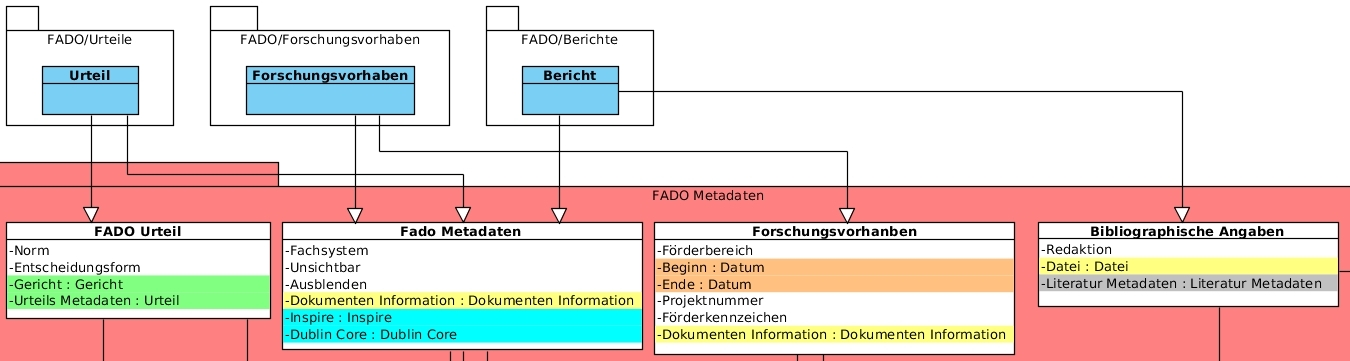
\includegraphics[width=16cm]{Bilder/Datenmodell/FADO-Metadaten.jpg}
\caption{FADO Metadaten}
\label{Fado Modell}
\centering
\end{figure}

\FloatBarrier
\subsection{DRS Metadaten / Bildarchiv Metadaten}\label{DRS Bildarchiv Metadaten}
Die Abbildung \ref{DRS und Bildarchiv Modell} zeigt die Datensammlungen des \ac{DRS} und des Bildarchives. Hier sind die obersten Datensammlungen zu sehen, welche zum einen eigene Attribute enthalten und zum anderen wieder auf untergeordnete Datensammlungen verweisen. 

Das Mapping zu den Metadaten ist im Abschnitt \ref{Metadatenmapping} zu finden.
\begin{figure}[!ht]
\centering
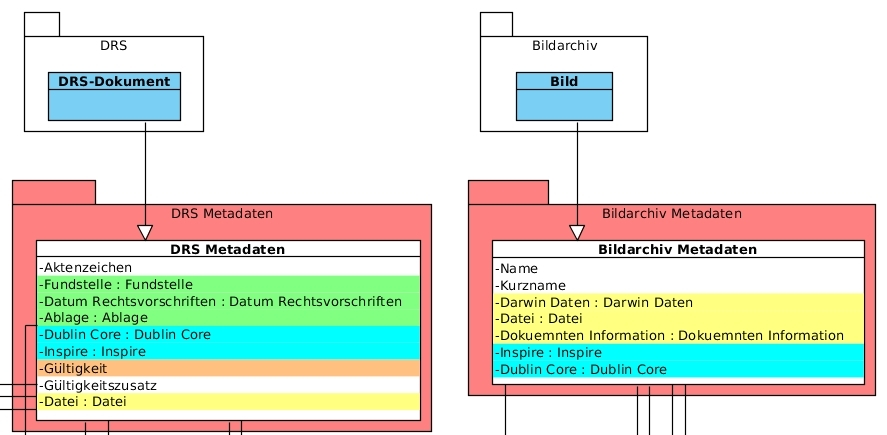
\includegraphics[width=12cm]{Bilder/Datenmodell/DRS-Bildarchiv-Metadaten.jpg}
\caption{DRS und Bildarchiv Metadaten}
\label{DRS und Bildarchiv Modell}
\centering
\end{figure}

\FloatBarrier
\subsection{ICT-ENSURE Metadaten}\label{ICT-ENSURE Metadaten}
Abbildung \ref{ICT-ENSURE Modell} zeigt die Hauptdatensammlungen der Metadaten f\"ur \ac{ICT-ENSURE}. Eine Besonderheit ist hier, dass die Datensammlung geteilt ist und zwar in \texttt{Artikel Metadaten}, welche die Metadaten zu einem Artikel enth\"alt und in \texttt{Konferenz}, welche die Metadaten zu einer Konferenz enth\"alt.

Alle farbig hinterlegten Verweise sind in den nachfolgenden Abschnitten genauer erkl\"art und das Mapping zwischen alten und neuen Namen ist im Abschnitt \ref{Metadatenmapping} zu finden.
\begin{figure}[!ht]
\centering
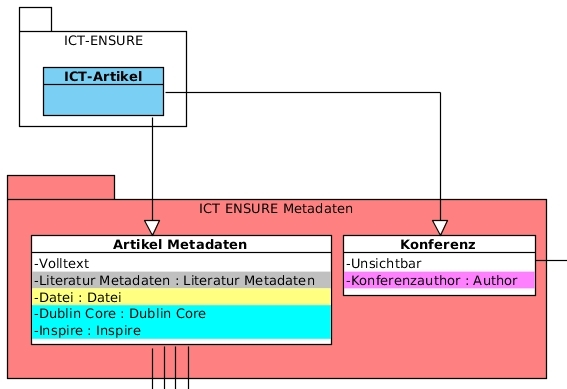
\includegraphics[width=8cm]{Bilder/Datenmodell/ICT-ENSURE-Metadaten.jpg}
\caption{ICT-ENSURE Metadaten}
\label{ICT-ENSURE Modell}
\centering
\end{figure}

\FloatBarrier
\subsection{Untergeordnete Datensammlungen}
In den nun folgenden Abschnitten werden die eben in den Abbildungen \ref{Fado Modell} bis \ref{ICT-ENSURE Modell} farbig hinterlegten Datensammlungen mit ihren Attributen genauer beschrieben, wenn die Bezeichnung nicht schon eindeutig sein sollte. 

\subsubsection{Gerichtbarkeit}
Im Package \texttt{Gerichtbarkeit}, welches in Abbildung \ref{Package Gerichtbarkeit} zu sehen ist, sind alle Datensammlung welche f\"ur gerichtliche Urteile, Beschl\"usse oder Richtlinien wichtig sind, zusammengefasst.

Die Datensammlungen \texttt{Gericht} und \texttt{Urteil} werden wie in Abbildung \ref{Fado Modell} zu sehen in der Datensammlung \texttt{FADO Urteil} verwendet.

Die Datensammlung \texttt{Gericht} stellt, wie der Name schon sagt, ein Gericht dar. Hierbei enth\"alt sie die Attribute \texttt{Standort} und \texttt{Art}. Im Attribut \texttt{Standort}, wird der Standort des Gerichts und im Attribut \texttt{Art} die Art des Gerichts, wie zum Beispiel "`Oberlandesgericht"' festgelegt. So ergibt sich f\"ur ein Gericht der Datensatz aus Standort und Art mit dessen Hilfe ein Datum nach der Art "`Oberlandesgericht Karlsruhe"' gebildet werden kann.

Der Datensatz \texttt{Urteil} enth\"alt die schon analysierten Attribute, welche das \ac{FADO}-System verwendet. Die Attribute \texttt{Vorgericht} und \texttt{Nachgericht} verweisen wiederum auf ein Gericht. Das Erscheinungsdatum enth\"alt eine Datensammlung des Typs \texttt{Datum}, welche im Abschnitt \ref{Grundlegenden Daten} genauer beschrieben ist.

\texttt{Fundstelle}, \texttt{Datum Rechtsvorschriften} und \texttt{Ablage} sind Datensammlungen, welche in der Sammlung \texttt{DRS Metadaten} vorkommen. Sie enthalten weitere Attribute zur Gerichtbarkeit, welche im \ac{DRS} ben\"otigt werden. (siehe Abschnitt \ref{DRS Bildarchiv Metadaten})

Eine Fundstelle hat die Attribute \texttt{Name}, \texttt{Jahr} und \texttt{Seite}, welche eine Fundstelle, wie sie im \ac{DRS} wiedergegeben wird, genauer beschreiben. 

Alle Attribute der Datensammlung \texttt{Datum Rechtsvorschriften} verweisen auf ein Datum, welches im Abschnitt \ref{Grundlegenden Daten} genauer beschrieben ist.

Die Datensammlung \texttt{Ablage} enth\"alt weitere Attribute, welche das \ac{DRS} zur Beschreibung seiner Dokumente verwendet.

Das Mapping zu den gegebenen \"Anderungen in den Namen, der Attribute, ist im Abschnitt \ref{Metadatenmapping} zu finden.
\begin{figure}[!ht]
\centering
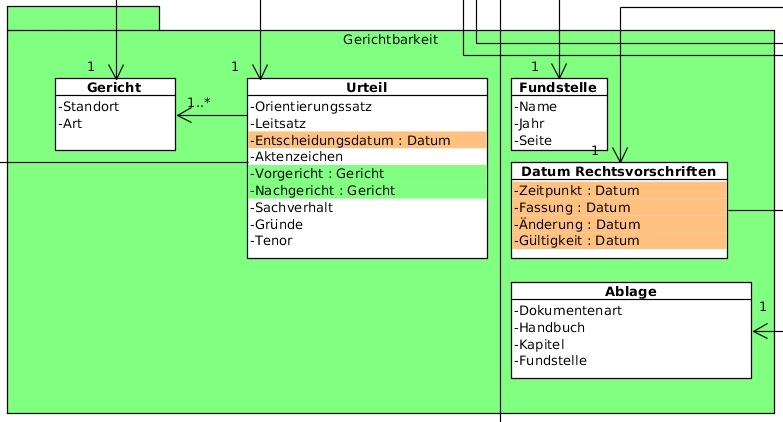
\includegraphics[width=11cm]{Bilder/Datenmodell/Package-Gerichtbarkeit.jpg}
\caption{Package Gerichtbarkeit}
\label{Package Gerichtbarkeit}
\centering
\end{figure}

\subsubsection{Bibliographie Metadaten}
Das Package \texttt{Bibliographie Metadaten}, welches in Abbildung \ref{Package Bibliographie} zu sehen ist, enth\"alt zwei Datensammlungen, welche sich mit der Beschreibung von Literatur befassen. 

Die wichtigsten Angaben stehen dabei in \texttt{Literatur Metadaten}, welche die Datensammlungen \texttt{Bibliographische Angaben} (Abbildung \ref{Fado Modell}) und \texttt{Artikel Metadaten} (Abbildung \ref{ICT-ENSURE Modell}) verwendet.

Die Attribute \texttt{Seitenanzahl}, \texttt{Abstract}, \texttt{Reihe}, \texttt{Bandnummer}, \texttt{Beginn Seite} und \texttt{End Seite} sind selbsterkl\"arend und werden deshalb nicht genauer beschrieben. Das Attribut \texttt{Kapitel} verweist auf die gleichnamige Datensammlung und enth\"alt wiederum Angaben zum Kapitel.

Die Attribute \texttt{PublikationsID} und \texttt{Dokumenten Information} verweisen auf Datensammlungen im Package \texttt{Abstrakte Metadaten}, welche im Abschnitt \ref{Abstrakte Metadaten} genauer beschrieben sind.
\begin{figure}[!ht]
\centering
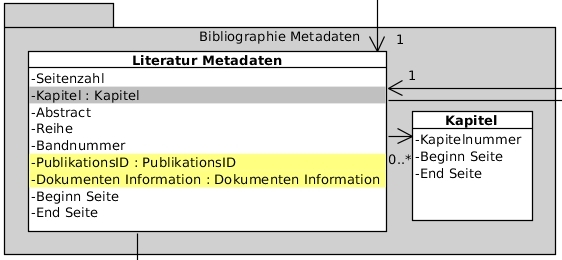
\includegraphics[width=9cm]{Bilder/Datenmodell/Package-Bibliographie.jpg}
\caption{Package Bibliographie}
\label{Package Bibliographie}
\centering
\end{figure}

\newpage
\subsubsection{Abstrakte Metadaten}\label{Abstrakte Metadaten}
\texttt{Abstrakte Metadaten} ist ein Package, welches Datensammlungen zu verschiedenen Themenbereichen enth\"alt und ist in Abbildung \ref{Package Abstrakte Metadaten} zu sehen. 

Die Datensammlung \texttt{Dokumenten Information} enth\"alt Attribute, welche Dokumente beschreiben. \texttt{Kommentar}, \texttt{Kurztitel}, \texttt{Kurzbeschreibung}, \texttt{Untertitel}, \texttt{Kurzname}, \texttt{Bemerkung} und \texttt{Version} sind selbsterkl\"arend. Das Attribut \texttt{Stand} verweist wieder auf ein \texttt{Datum}, welches im Abschnitt \ref{Grundlegenden Daten} beschrieben ist.

\texttt{Datei} ist eine Datensammlung, welche verschiedene Attribute f\"ur eine "`reale"' Datei bereith\"alt. Die Attribute \texttt{Gr\"o\ss{}e} und \texttt{Verf\"ugbar} ben\"otigen daher keiner weiteren Beschreibung, die beiden Verweise \texttt{URL} und \texttt{Technische Daten} schon. 

Der Verweis \texttt{URL} beschreibt, wie der Name schon sagt, eine URL, unter der die beschriebene Datei zu finden ist (siehe Abschnitt \ref{Grundlegenden Daten}). \texttt{Technische Daten} ist ein Verweis, welcher die Datei noch einmal genauer beschreibt (siehe Abschnitt \ref{Abstrakte Standard Metadaten}).

\texttt{PublikationsID} beschreibt eine ID, wobei hier das Format und die genaue Art der ID dem Benutzer \"uberlassen wird. Mit dem Attribut \texttt{Art} wird festgelegt, um welche standardisierte Form von ID es sich handelt. \texttt{Nummer} enth\"alt dann die eigentliche ID, welche das Dokument besitzt. Hier k\"onnen somit verschiedenste Systeme vom Benutzer frei verwendet werden.

Im Abschnitt \ref{Darwin Core} wurde der "`Darwin Core"'-Standard genauer untersucht. Es zeigte sich nun jedoch, dass der Einsatz von "`Darwin Core"' zu umfangreich w\"are, da nur ein Bruchteil der zur Verf\"ugung stehenden Attribute \"uberhaupt von der \ac{LUBW} im Bildarchiv verwendet werden.

Aus diesem Grund wurde in R\"ucksprache mit der Arbeitsgruppe entschieden, eine eigene Datensammlung zu erstellen, welche die wenigen ben\"otigten Attribute beinhaltet. Daraus entstand bei der Erarbeitung des Datenmodells die Datensammlung \texttt{Darwin Daten}, welche zwei Attribute enth\"alt. Zum eine den lateinischen Namen und zum anderen den deutschen Namen. Weitere Biodaten werden nicht verwendet, da sie keine Verwendung in den Systemen finden.

Die letzten beiden Datensammlungen im Package sind \texttt{Person}, welche einen Namen und Vornamen enth\"alt und \texttt{Land}, weche den Landesnamen und die ISO-Abk\"urzung nach ISO 3166-1 beinhaltet.

Beide Datensammlungen k\"onnten durchaus weitere Attribute enthalten, dies ist jedoch nicht notwendig, da in den Systemen keine weiteren Daten zur Verf\"ugung gestellt werden.

\begin{figure}[!ht]
\centering
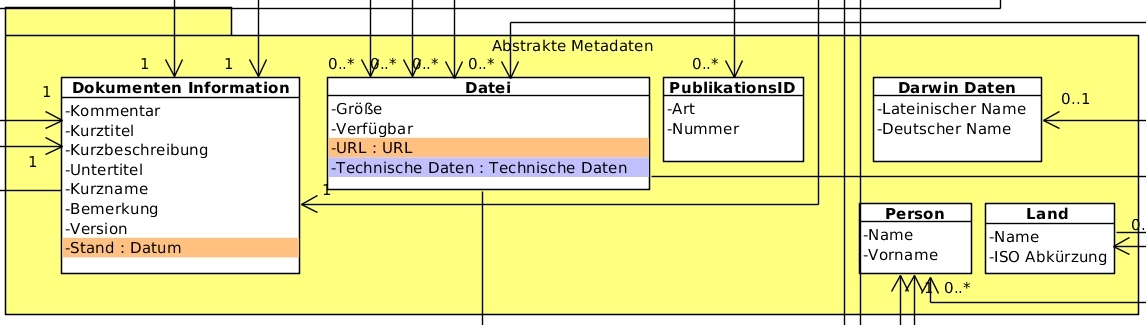
\includegraphics[width=15cm]{Bilder/Datenmodell/Package-Abstrakte-Metadaten.jpg}
\caption{Package Abstrakte Metadaten}
\label{Package Abstrakte Metadaten}
\centering
\end{figure}

\subsubsection{Standard Metadaten}
Das Package \texttt{Standard Metadaten} enth\"alt Datensammlungen f\"ur standardisierte Metadaten. Im Speziellen sind das \texttt{Inspire} und \texttt{Dublin Core}, welche in den Abschnitten \ref{INSPIRE} und \ref{Dublin Core} schon analysiert wurden.

Die Datensammlungen im Package enthalten keine eigenen Attribute, sondern verweisen lediglich auf die in ihnen enthaltenen Datensammlungen, welche im Abschnitt \ref{Abstrakte Standard Metadaten} genauer beschrieben werden. Ausnahme hierbei ist das Datum, welches \texttt{Inspire} inne hat und einen Verweis in das Package \texttt{Grundlegende Metadaten} darstellt. (siehe Abschnitt \ref{Grundlegenden Daten})

Im Anhang \ref{Bilder des Datenmodells} ist die Abbildung \ref{Package Abstrakte Metadaten} noch einmal vergr\"o\ss{}ert zu finden.

\begin{figure}[!ht]
\centering
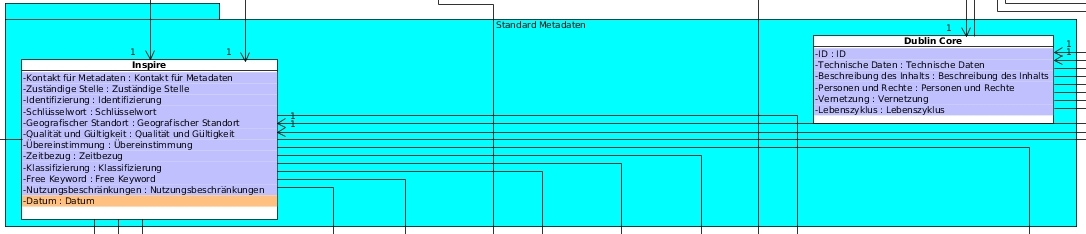
\includegraphics[width=16cm]{Bilder/Datenmodell/Package-Standard-Metadaten.jpg}
\caption{Package Standard Metadaten}
\label{Package Standard Metadaten}
\centering
\end{figure}



\subsubsection{Abstrakte Standard Metadaten}\label{Abstrakte Standard Metadaten}
\texttt{Abstrakte Standard Metadaten} ist das Package, in welchem alle Datensammlungen zu finden sind, die in den Sammlungen im Package \texttt{Standard Metadaten} verwendet werden.

In Abbildung \ref{Package Abstrakte Standard Metadaten Teil 1} sind die Datensammlungen zu sehen, welche bei \ac{INSPIRE} Verwendung finden. Sie werden an keiner anderen Stelle referenziert, da die \texttt{Inspire}-Datensammlung in den jeweiligen Obersammlungen anzutreffen ist. (siehe Abschnitt \ref{FADO Metadaten} - \ref{ICT-ENSURE Metadaten} und Abbildung \ref{Fado Modell} - \ref{ICT-ENSURE Modell}) Im Abschnitt \ref{INSPIRE} wurde dieser Standard schon einmal angesprochen und seine Funktionalit\"at erkl\"art.

In der Datensammlung \texttt{Kontakt f\"ur Metadaten} sind die Attribute \texttt{Name der Stelle} und \texttt{EMail Adresse} vorhanden, mit denen der Ansprechpartner der Datei angegeben wird. \"Uber \texttt{Zust\"andige Stelle} wird mit dem Attribut \texttt{Funktion der Stelle} und dem Verweis \texttt{Zust\"andige Stelle} die Stelle, welche die Datei ver\"offentlicht hat, genauer beschrieben.

\texttt{Identifizierung} gibt mit den Attributen \texttt{Ressourcenbezeichnung}, \texttt{Ressourcen\"uberblick}, \texttt{Ressourcenverweis} und \texttt{Ressourcensprache} die verwendete Ressource genauer an. Zus\"atzlich lassen sich \texttt{Bezeichner} einf\"ugen. Alle Attribute sind Freitexte und k\"onnen von der jeweiligen "`Stelle"', welche die Datei ver\"offentlicht, vergeben werden. Einzig \texttt{Bezeichner} und \\\texttt{Ressourcensprache} sind Verweise und werden im Abschnitt \ref{Grundlegenden Daten} genauer beschrieben.

\texttt{Zeitbezug} enth\"alt verschiedene Daten, welche auf die Sammlung \texttt{Datum}, im Abschnitt \ref{Grundlegenden Daten}, verweisen. Im Speziellen sind das \texttt{Erstellungsdatum}, \texttt{Datum der Ver\"offentlichung} und \texttt{Datum der letzten \"Anderung}. Zus\"atzlich enth\"alt die Sammlung noch einen Verweis auf \texttt{Zeitliche Ausdehnung}, welche im Abschnitt \ref{Grundlegenden Daten} beschrieben ist.

Die Datensammlung \texttt{Klassifizierung} enth\"alt eine \texttt{Themenkategorie}, welche vorgegeben ist und zum Beispiel im Editor f\"ur \ac{INSPIRE} gefunden werden kann\footnote{\url{http://inspire-geoportal.ec.europa.eu/editor/}}.

Schl\"usselw\"orter sind in \ac{INSPIRE} fest vorgegeben und k\"onnen ebenfalls im Editor der \ac{EU} eingesehen werden. Diese Schl\"usselw\"orter werden im Model in der Datensammlung \texttt{Schl\"usselwort} abgebildet.

Zus\"atzlich zu den vorgegeben Schl\"usselw\"ortern bietet \ac{INSPIRE} auch die M\"oglichkeit, eigene, frei w\"ahlbare Schl\"usselw\"orter, zu erstellen. Im Metadatenmodell ist dies in der Datensammlung \texttt{Free  Keyword} umgesetzt. Diese enth\"alt zum einen den Wert des Schl\"ussels und zum anderen einen Verweis \texttt{Herkunft des Vokabulars}, welcher im Abschnitt \ref{Grundlegenden Daten} genauer beschrieben wird.

Die Datensammlung \texttt{Geografischer Standort} beinhaltet Attribute f\"ur die vier Koordinaten, welche bei der Navigation auf der Erde n\"otig sind und zwar \texttt{N Breitengrad}, \texttt{E L\"angengrad}, \texttt{S Breitengrad} und \texttt{W L\"angengrad}. Hierbei werden zur Standortbeschreibung immer nur zwei ben\"otigt, was davon abh\"angig ist, auf welcher Erdseite der Punkt sich befindet. Zus\"atzlich gibt ein Attribut das Land beziehungsweise die L\"ander (\texttt{Countries}) und den Ort (\texttt{Bezeichnung}) an.

\texttt{Qualit\"at und G\"ultigkeit} enth\"alt wiederum das Freitext-Attribut \texttt{Herkunft} und den Verweis \texttt{R\"aumliche Aufl\"osung}, welches im Abschnitt \ref{Grundlegenden Daten} genauer beschrieben wird.

\texttt{Nutzungsbeschr\"ankungen} enth\"alt die Freitext-Attribute \texttt{Bedingungen f\"ur Zugang} und \\\texttt{Beschr\"ankung des \"offentlichen Zugangs}. Au\ss{}erdem ist ein Verweis auf die Lizenz angegeben, welcher im Abschnitt \ref{Urheber Metadaten} beschrieben wird.
Es werden somit alle Bestimmungen f\"ur einen Zugang und Nutzung der Datei genauer erkl\"art.

\texttt{\"Ubereinstimmung} ist eine Datensammlung f\"ur die Quellenangabe. Hierbei wird die Quelle im Attribut \texttt{Specifications} angegeben. Zus\"atzlich dazu ist ein Attribut \texttt{Grad} angegeben, welches beinhaltet ob die Quelle konform ist oder nicht. \"Uber den Verweis \texttt{Datum mit Typ} wird angegeben, von wann die Quelle ist. (siehe Abschnitt \ref{Grundlegenden Daten})

Im Anhang \ref{Bilder des Datenmodells} ist die Abbildung \ref{Package Abstrakte Standard Metadaten Teil 1} noch einmal vergr\"o\ss{}ert zu finden.

\begin{figure}[!ht]
\centering
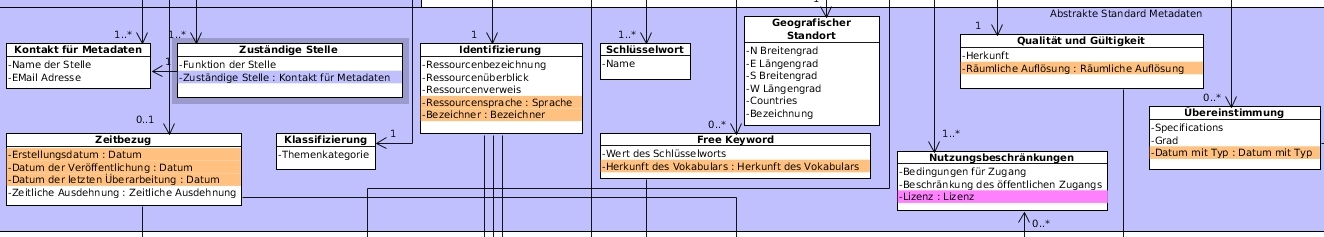
\includegraphics[width=16cm]{Bilder/Datenmodell/Package-Abstrakte-Metadaten-Teil1.jpg}
\caption{Package Abstrakte Standard Metadaten Teil 1 \ac{INSPIRE}}
\label{Package Abstrakte Standard Metadaten Teil 1}
\centering
\end{figure}



In Abbildung \ref{Package Abstrakte Standard Metadaten Teil 2} sind die Datensammlungen aufgezeigt, welche "`Dublin Core"' verwendet. Diese befinden sich ebenfalls im Package \texttt{Abstrakte Standard Metadaten}. "`Dublin Core"' wurde im Abschnitt \ref{Dublin Core} schon analysiert und nun im Modell verwendet.

Alle nun folgenden Attribute stammen aus der Norm und wurden im Inhaltsumfang gegebenenfalls noch weiter eingeschr\"ankt und spezifiziert.

\texttt{ID} gibt mit dem Attribut \texttt{Identifier} eine eindeutige ID des Dokuments an, welche im System einmalig vergeben wird. \"Uber diese ID sollen sp\"ater eindeutige Verweise m\"oglich sein.

Die Sammlung \texttt{Technische Daten} beinhaltet die Attribute \texttt{Format} und \texttt{Typ}. Zus\"atzlich wird ein Verweis auf eine \texttt{Sprache} gemacht (siehe Abschnitt \ref{Grundlegenden Daten}). \"Uber diese Felder wird eine "`reale"' Datei genauer beschrieben.

Die Beschreibung des Inhalts wird mit der gleichnamigen Datensammlung \texttt{Beschreibung des Inhalts} umgesetzt. Hierf\"ur stehen die Attribute \texttt{Titel}, \texttt{Thema}, \texttt{Reichweite} und \texttt{Beschreibung} zur Verf\"ugung, welche eindeutig sind.

\texttt{Personen und Rechte} hat die beiden Attribute \texttt{Rechteverwerter} und \texttt{Herkunft}. Zus\"atzlich sind die beiden Verweise \texttt{Urheber} und \texttt{Herausgeber} zu finden, welche im Abschnitt \ref{Urheber Metadaten} genauer erl\"autert werden. Der Verweis \texttt{Mitarbeiter} zeigt auf die Datensammlung Person und ist im Abschnitt \ref{Abstrakte Metadaten} aufgef\"uhrt.

Mit der Datensammlung \texttt{Vernetzung} kommen die vier Attribute \texttt{Quelle}, \texttt{Verweis}, \texttt{Zielgruppe} und \texttt{Lehrmethode}. Die Felder \texttt{Quelle}, \texttt{Verweis} und \texttt{Zielgruppe} sind eindeutig und werden an dieser Stelle nicht weiter erl\"autert. Das Attribut \texttt{Lehrmethode} gibt an, mit welcher Lehrmethode sich die Daten am besten vermitteln lassen beziehungsweise wie sie vermittelt werden.

\texttt{Lebenszyklus} gibt einen Verweis auf ein Datum (siehe Abschnitt \ref{Grundlegenden Daten}) und ein Attribut \texttt{Zustand}, mit dem sich beschreiben l\"asst, um was f\"ur ein Datum es sich handelt.

\begin{figure}[!ht]
\centering
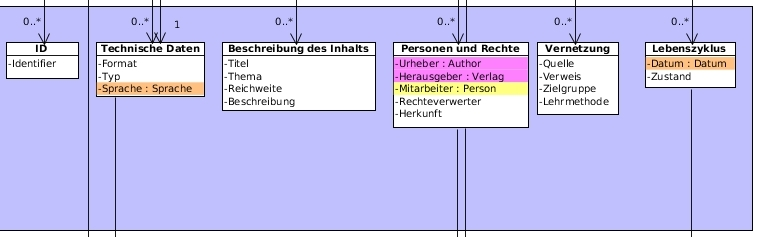
\includegraphics[width=13cm]{Bilder/Datenmodell/Package-Abstrakte-Metadaten-Teil2.jpg}
\caption{Package Abstrakte Standard Metadaten Teil 2 "`Dublin Core"'}
\label{Package Abstrakte Standard Metadaten Teil 2}
\centering
\end{figure}

\FloatBarrier
\subsubsection{Grundlegenden Daten} \label{Grundlegenden Daten}
Das Package \texttt{Grundlegende Daten}, welches in Abbildung \ref{Package Grundlegende Daten} zu sehen ist, beinhaltet grundlegende Datensammlungen, welche an vielen Stellen im Modell verwendet werden. 

Die Datensammlung \texttt{Datum} enth\"alt die eindeutigen Attribute \texttt{Tag}, \texttt{Monat} und \texttt{Jahr}. Die Sammlung wird vielfach verwendet, wovon auch die Pfeile zur Sammlung in der Abbildung \ref{Package Grundlegende Daten} zeugen.

\texttt{Sprache} enth\"alt lediglich das eine Attribut \texttt{Name}, in welchem die Sprache des Dokuments angegeben wird.

\texttt{URL} enth\"alt ebenfalls nur ein Attribut \texttt{Link}, welches einen internen oder externen Link repr\"asentiert.

Die Sammlung \texttt{Bezeichner} enth\"alt die Attribute \texttt{Code} und \texttt{Namensraum}. Im \ac{INSPIRE}-Standard gibt der \texttt{Code} eine eindeutige ID an, welche durch den \texttt{Namensraum} eingeschr\"ankt und genauer spezifiziert wird. (siehe Abschnitt \ref{Abstrakte Standard Metadaten})

Mit der Datensammlung \texttt{Herkunft des Vokabulars} wird angegeben, aus welchem Vokabular das frei gew\"ahlte Schl\"usselwort stammt. Zus\"atzlich wird ein Datum verlangt, wann das Schl\"usselwort entstand, ge\"andert oder ver\"offentlicht wurde, was mit Hilfe des Attributs \texttt{Datentyp} geschieht.

\texttt{Zeitliche Ausdehnung} ist eine Sammlung, welche ein \texttt{Anfangsdatum} und ein \texttt{Enddatum} als Verweis auf die Sammlung \texttt{Datum} enth\"alt.

\texttt{R\"aumliche Aufl\"osung} enth\"alt drei Attribute und zwar \texttt{\"Aquivalenter Ma\ss{}stab}, \\\texttt{Aufl\"osungsabstand} und \texttt{L\"angeneinheit}. Sie werden ben\"otigt, um eine genaue geografische Aufl\"osung des Standortes zu gew\"ahrleisten.


\begin{figure}[!ht]
\centering
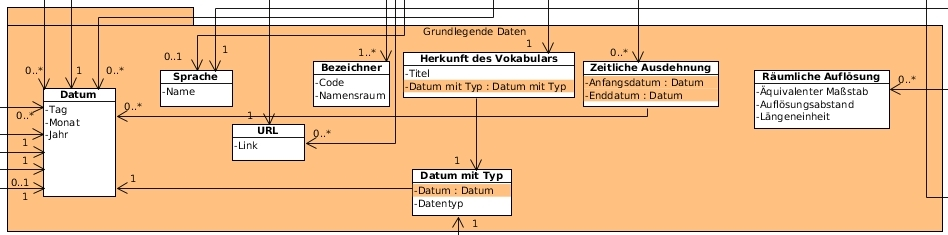
\includegraphics[width=16cm]{Bilder/Datenmodell/Package-Grundlegende-Daten.jpg}
\caption{Package Grundlegende Daten}
\label{Package Grundlegende Daten}
\centering
\end{figure}

\FloatBarrier
\subsubsection{Urheber Metadaten} \label{Urheber Metadaten}
Im Package \texttt{Urheber Metadaten} sind Datensammlungen zusammengefasst, welche sich mit der Urheberschaft von Dateien befassen.

\texttt{Verlag} enth\"alt die Attribute \texttt{Name} und \texttt{Ort}. Zus\"atzlich einen Verweis auf die Datensammlung \texttt{Land} aus dem Package \texttt{Abstrakte Metadaten}, welches im Abschnitt \ref{Abstrakte Metadaten} beschrieben ist. Au\ss{}erdem ist ein Verweis auf eine \texttt{Lizenz} zu finden, welche sich im selben Package befindet.

Die Datensammlung \texttt{Lizenz} hat das Attribut \texttt{Lizenzart}, in welchem der Lizenzname festgehalten wird. Au\ss{}erdem ist ein Verweis auf eine \texttt{Person} vorhanden, welche den Lizenzinhaber ausweist. (siehe Abschnitt \ref{Abstrakte Metadaten})

Der \texttt{Autor} enth\"alt das Attribut \texttt{Institution} und die Verweise auf \texttt{Person} und \texttt{Land}, welche zum Package \texttt{Abstrakte Metadaten} geh\"oren und im Abschnitt \ref{Abstrakte Metadaten} beschrieben sind.

Das Attribut \texttt{Institution} k\"onnte weiter aufgeschl\"usselt werde, dies ist jedoch nicht sinnvoll, da die Informationen von den Systemen nicht verarbeitet werden.

\begin{figure}[!ht]
\centering
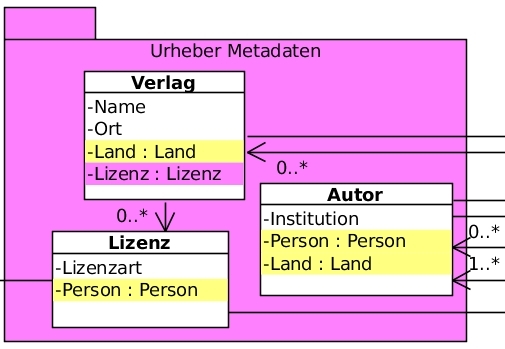
\includegraphics[width=6cm]{Bilder/Datenmodell/Package-Urheber-Metadaten.jpg}
\caption{Package Urheber Metadaten}
\label{Package Urheber Metadaten}
\centering
\end{figure}

\subsection{Metadatenmapping im neuen Modell}\label{Metadatenmapping}
Da sich durch das Zusammenfassen und das Aufstellen eines \"ubergreifenden Modells der Metadaten einige Bezeichnungen von Attributen ge\"andert haben, wird in diesem Abschnitt nun das Mapping zwischen dem alten und neuen Modell beschrieben. Hierf\"ur werden die Metadaten der einzelnen Systeme aufgeschl\"usselt.

\subsubsection{Metadatenmapping FADO}\label{Fado Mapping}
Im folgenden Abschnitt sind die Metadaten des \ac{FADO}-Systems in Tabellenform aufgelistet. Die Auflistung der Metadaten und ihrer Wertebereiche ist im Anhang \ref{Metadaten der LUBW Fachsysteme} zu finden.

In den dargestellten Tabellen \ref{Fado Mapping Urteile}, \ref{Fado Mapping Forschungsvorhaben} und \ref{Fado Mapping Berichte} sind die alten Namen neben den neuen Namen zu finden. Die zus\"atzliche dritte Spalte listet auf, in welcher Datensammlung die neuen Attribute zu finden sind.

\begin{table}[!ht]
\begin{center}
\begin{tabular}{|l|l|l|}
\hline
Alt: & Neu: & Klasse: \\ \hline
Fachsystem & Fachsystem & FADO-Metadaten \\ \hline
ID & ID & ID \\ \hline
Titel & Titel & Beschreibung des Inhalts \\ \hline
Tenor & Tenor & Urteils Metadaten \\ \hline
Kommentar & Beschreibung & Beschreibung des Inhalts \\ \hline
Orientierungssatz & Orientierungssatz & Urteils Metadaten \\ \hline
Norm & Norm & Urteil \\ \hline
Leitsatz & Leitsatz & Urteils Metadaten \\ \hline
Gericht & Gericht & Urteil \\ \hline
Entscheidungsform & Entscheidungsform & Urteil \\ \hline
Entscheidungsdatum & Entscheidungsdatum & Urteils Metadaten \\ \hline
Aktenzeichen & Aktenzeichen & Urteils Metadaten \\ \hline
Vorgericht & Vorgericht & Urteils Metadaten \\ \hline
Nachgericht & Nachgericht & Urteils Metadaten \\ \hline
Sachverhalt & Sachverhalt & Urteils Metadaten \\ \hline
Gr�nde & Gr�nde & Urteils Metadaten \\ \hline
Unsichtbar & Unsichtbar & FADO-Metadaten \\ \hline
Ausblenden & Ausblenden & FADO-Metadaten \\ \hline
\end{tabular}
\caption{Mapping der FADO Attribute f�r Urteile}
\label{Fado Mapping Urteile}
\end{center}
\end{table}

\begin{table}[htbp]
\begin{center}
\begin{tabular}{|l|l|l|}
\hline
Alt: & Neu: & Klasse: \\ \hline
Fachsystem & Fachsystem & FADO-Metadaten \\ \hline
ID & ID & ID \\ \hline
Titel & Titel & Beschreibung des Inhalts \\ \hline
Kurzbeschreibung & Kurzbeschreibung & Dokumenten Information \\ \hline
Kommentar & Kommentar & Dokumenten Information \\ \hline
F�rderbereich & F�rderbereich & Forschungsvorhaben \\ \hline
Beginn & Beginn & Forschungsvorhaben \\ \hline
Ende & Ende & Forschungsvorhaben \\ \hline
Projektnummer & Projektnummer & Forschungsvorhaben \\ \hline
F�rderkennzeichen & F�rderkennzeichen & Forschungsvorhaben \\ \hline
Unsichtbar & Unsichtbar & FADO-Metadaten \\ \hline
Ausblenden & Ausblenden & FADO-Metadaten \\ \hline
\end{tabular}
\caption{Mapping der FADO Attribute f�r Forschungsvorhaben}
\label{Fado Mapping Forschungsvorhaben}
\end{center}
\end{table}

\FloatBarrier
Die Attribute \texttt{HTML-Datei}, \texttt{PDF-Datei}, \texttt{Weitere Datei} und \texttt{Format dieser Datei} werden komplett durch die Datensammlung \texttt{Datei} ersetzt, wie in der Tabelle \ref{Fado Mapping Berichte} zu sehen ist.

Da w\"ahrend der Bearbeitung der Metadaten eine neue Version des \ac{FADO}-Systems verabschiedet wurde, ergaben sich einige \"Anderungen in den Metadaten. Hierdurch entfallen die Attribute \texttt{Seiten (von-bis)}, \texttt{Shoprelevant}, \texttt{Shoplink} und \texttt{Preis} ersatzlos.

\begin{table}[htbp]
\begin{center}
\begin{tabular}{|l|l|l|}
\hline
Alt: & Neu: & Klasse: \\ \hline
Fachsystem & Fachsystem & FADO-Metadaten \\ \hline
ID & ID & ID \\ \hline
Titel & Titel & Beschreibung des Inhalts \\ \hline
Kurzbeschreibung & Kurzbeschreibung & Dokumenten Information \\ \hline
Kommentar & Kommentar & Dokumenten Information \\ \hline
Kurztitel & Kurztitel & Dokumenten Information \\ \hline
Untertitel & Untertitel & Dokumenten Information \\ \hline
Fachthema & Thema & Beschreibung des Inhalts \\ \hline
Herausgeber & Herausgeber & Personen und Rechte \\ \hline
Redaktion & Redaktion & Bibliographische Angaben \\ \hline
Version & Version & Dokumenten Information \\ \hline
Stand & Stand & Dokumenten Information \\ \hline
Seitenzahl & Seitenzahl & Literatur Metadaten \\ \hline
Seite (von-bis) & ENTF�LLT & ENTF�LLT \\ \hline
Reihe & Reihe & Literatur Metadaten \\ \hline
Bandnummer & Bandnummer & Literatur Metadaten \\ \hline
ISSN & PublikationsID & Literatur Metadaten \\ \hline
ISBN & PublikationsID & Literatur Metadaten \\ \hline
Preis & ENTF�LLT & ENTF�LLT \\ \hline
Medium & Format & Technische Daten \\ \hline
Shoprelevant & ENTF�LLT & ENTF�LLT \\ \hline
Shoplink & ENTF�LLT & ENTF�LLT \\ \hline
HTML-Datei & Datei & Bibliographische Angaben \\ \hline
PDF-Datei & Datei & Bibliographische Angaben \\ \hline
Weitere Datei & Datei & Bibliographische Angaben \\ \hline
Format dieser Datei & Format & Technische Daten \\ \hline
Unsichtbar & Unsichtbar & FADO-Metadaten \\ \hline
Ausblenden & Ausblenden & FADO-Metadaten \\ \hline
\end{tabular}
\end{center}
\caption{Mapping der FADO Attribute f�r Berichte}
\label{Fado Mapping Berichte}
\end{table}

\FloatBarrier
\subsubsection{Metadatenmapping DRS}\label{DRS Mapping}
Wie eben schon im Abschnitt \ref{Fado Mapping} erkl\"art, wurden die Namen der Attribute auch f\"ur das \ac{DRS} ge\"andert. Die alte Bezeichnung ist in der linken Spalte, der neue Name im Modell in der mittleren Spalte und die zugeh\"orige Datensammlung in der rechten Spalte, in der Tabelle \ref{DRS Mapping Tabelle}, zu finden. 

Die Auflistung der Metadaten und ihrer Wertebereiche ist im Anhang \ref{Anhang Metadaten des DRS} zu finden.

\begin{table}[htbp]
\begin{center}
\begin{tabular}{|l|l|l|}
\hline
Alt: & Neu: & Klasse: \\ \hline
G�ltigkeit & G�ltigkeit / G�ltigkeitszusatz & DRS-Metadaten \\ \hline
Titel & Titel & Beschreibung des Inhalts \\ \hline
Aktenzeichen & Aktenzeichen & DRS-Metadaten \\ \hline
Kurz-Titel & Kurztitel & Dokumenten Information \\ \hline
Dokumentart & Dokumentart & Ablage \\ \hline
Herausgeber & Herausgeber & Personen und Rechte \\ \hline
Erscheinungsort & Herkunft & Personen und Rechte \\ \hline
Handbuch & Handbuch & Ablage \\ \hline
Kapitel & Kapitel & Ablage \\ \hline
Fundstelle & Fundstelle & Ablage \\ \hline
Fassung & Fassung & Datum Rechtsvorschriften \\ \hline
�nderung & �nderung & Datum Rechtsvorschriften \\ \hline
Gr��e & Gr��e & Datei \\ \hline
Formate & Format & Technische Daten \\ \hline
\end{tabular}
\end{center}
\caption{Mapping der DRS Attribute }
\label{DRS Mapping Tabelle}
\end{table}


\subsubsection{Metadatenmapping Bildarchiv}\label{Bildarchiv Mapping}
Auch die Metadaten des Bildarchivs mussten zum Teil umbenannt werden um ein einheitliches Modell zu erstellen. Wie in dem Abschnitten \ref{Fado Mapping} und \ref{DRS Mapping} ist die Tabelle \ref{Bildarchiv Mapping Tabelle} nach dem gleichen Muster aufgebaut. Links die alten Namen, in der Mitte die neuen Namen und Rechts die zugeh\"orige Datensammlung.

Im alten Attribut \texttt{Bemerkung} steht der Name des biologischen Objekts in deutsch und lateinisch, dies wird im neuen System durch die Datensammlung \texttt{Darwin Daten} getrennt verwaltet und gespeichert, was ein Abrufen der einzelnen Attribute deutlich vereinfacht.

Die Auflistung der Metadaten und ihrer Wertebereiche ist im Anhang \ref{Anhang Metadaten des Bildarchivs} zu finden.

\begin{table}[htbp]
\begin{center}
\begin{tabular}{|l|l|l|}
\hline
Alt: & Neu: & Klasse: \\ \hline
Objektart & Thema & Beschreibung des Inhalts \\ \hline
Objektname & Lateinischer Name & Darwin Daten \\ \hline
ID & ID & ID \\ \hline
URL & URL & Datei \\ \hline
Dateityp & Format & Technische Daten \\ \hline
Name & Name & Bildarchiv-Metadaten \\ \hline
Kurzname & Kurzname & Bildarchiv-Metadaten \\ \hline
Erstellt am & Datum & Lebenszyklus \\ \hline
Autor & Urheber & Personen und Rechte \\ \hline
Besitzer & Rechteverwerter & Personen und Rechte \\ \hline
Bemerkung & Darwin Daten & Darwin Daten \\ \hline
\end{tabular}
\end{center}
\caption{Mapping der Bildarchiv Attribute}
\label{Bildarchiv Mapping Tabelle}
\end{table}

\FloatBarrier
\subsubsection{Metadatenmapping ICT-ENSURE}
Die Tabelle \ref{ICT-ENSURE Mapping Tabelle} folgt dem Schema aus den Abschnitten \ref{Fado Mapping}, \ref{DRS Mapping} und \ref{Bildarchiv Mapping}.

Dadurch, dass die Metadaten der \ac{ICT-ENSURE} urspr\"unglich in einer relationalen Datenbank abgelegt wurden, entfallen hier nun einige Attribute, \"uber die fr\"uher die Relationen abgebildet wurden.

Die Auflistung der Metadaten und ihrer Wertebereiche ist im Anhang \ref{Metadaten der ICT-ENSURE} zu finden.

\begin{table}[htbp]
\begin{center}
\begin{tabular}{|l|l|l|}
\hline
Alt: & Neu: & Klasse: \\ \hline
Editor & Konferenzautor & Konferenz \\ \hline
Publisher & Herausgeber & Personen und Rechte \\ \hline
Year of Publishing & Datum & Lebenszyklus \\ \hline
ISBN & PublikationsID & Literatur Metadaten \\ \hline
Conferenc & Konferenztitel & Konferenz \\ \hline
Editor & Urheber & Personen und Rechte \\ \hline
Publisher & ENTF�LLT & ENTF�LLT \\ \hline
Year of Pblishing & ENTF�LLT & ENTF�LLT \\ \hline
ISBN & ENTF�LLT & ENTF�LLT \\ \hline
Conferenc & Thema & Beschreibung des Inhalts \\ \hline
Name & Titel & Beschreibung des Inhalts \\ \hline
Konferenz & ENTF�LLT & ENTF�LLT \\ \hline
Kapitel & ENTF�LLT & ENTF�LLT \\ \hline
Author & ENTF�LLT & ENTF�LLT \\ \hline
Dateityp & Format & Technische Daten \\ \hline
Titel & ENTF�LLT & ENTF�LLT \\ \hline
Sprache & Ressourchensprache & Sprache \\ \hline
Beginn Seite & Beginn Seite & Literatur Metadaten \\ \hline
End Seite & End Seite & Literatur Metadaten \\ \hline
Schl�sselw�rter & Sch�sselwort / Free Keyword & Inspire \\ \hline
Abstract & Abstract & Literatur Metadaten \\ \hline
Volltext & Volltext & Artikel-Metadaten \\ \hline
\end{tabular}
\end{center}
\caption{Mapping der \ac{ICT-ENSURE} Attribute }
\label{ICT-ENSURE Mapping Tabelle}
\end{table}

\newpage
\section{Technologievergleich}
F\"ur das Projekt soll ein \ac{DMS} verwendet werden, mit welchem sich die vorhandenen Dokumente der \ac{LUBW}, der \ac{GAA} und der \ac{ICT-ENSURE} einfach und bequem in einem System verwalten lassen. Hierbei soll kein \ac{ECM}-Tool vom Grund auf neu entwickelt werden. 

Es soll wie in der Aufgabenstellung im Lastenheft im Kapitel \ref{Lastenheft} festgehalten ein passendes Tool gesucht werden, welches die gegebenen Anforderungen bestm\"oglich erf\"ullt. Die Betrachtung erfolgt hierbei unter der Beachtung g\"angiger Standards.

Das \ac{ECM}-Tool, welches f\"ur das Projekt verwendet werden soll, muss die im folgenden genannten Eigenschaften aufweisen:

\begin{itemize}
 \item Grundlegende Metadatenstandards wie "`Dublin Core"' oder "`EXIF"' m\"ussen unterst\"utzt werden. (siehe Kapitel \ref{Analyse Datenbestaende})
 \item Das System muss alle Fachsysteme der \ac{LUBW} vereinen, welche im Kapitel \ref{Stand der Technik} beschriebenen sind.
 \item Metadaten sollten vom System systematisch gegliedert werden k\"onnen, wie es im Kapitel \ref{Erstellung eines Datenkonzepts} erarbeitet wurde
 \item Das verwendete \ac{ECM}-Tool sollte m\"oglichst viele Schnittstellen bieten, \"uber welche die Daten abgerufen werden
 \item Dateien m\"ussen Versioniert werden k\"onnen
%  \item Die Betrachtung 
\end{itemize}

Im folgenden werden nun verschiedene namenhafte \ac{ECM}-Tools vorgestellt und auf die eben genannten Eigenschaften gepr\"uft. Am Ende werden die M\"oglichkeiten verglichen und die beste ausgew\"ahlt.


% Damit ein Tool f\"ur dieses Projekt ausgew\"ahlt werden kann, muss es die im folgenden beschriebenen Eigenschaften beinhalten.

% Das Lastenheft im Kapitel \ref{Lastenheft} besagt, dass im Verlauf der Arbeit ein \ac{ECM}-Tool verwendet werden soll,
\subsection{Agorum Core}
Bei "`Agorum Core"' handelt es sich um eine Open Source Software, welche von der Baden W\"urttembergischen Firma "`agorum Software"' stammt. "`Agorum Core"' wird in mehrerem Varianten angeboten. Zum einem gibt es eine freie Version, welche ohne Lizenzkosten genutz werden kann, zum anderem gibt es mehrere kostenpflichtige Versionen die in ihrem Versionsumfang variieren. \cite{agorum_home} 

Agorum bietet viele Funktionen an, welche jedoch in der freien Version nicht vorhanden sind. Um die zus\"atzlichen Funktionen zu nutzen, muss entweder die ents\"prechende Version, welche die Funktion enth\"alt gekauft werden oder es muss die entsprechende Funktion hinzugebucht werden.
Somit entstehen auf jedenfall Kosten, wenn die freie Version von "`Agorum Core"' nicht die gew\"unschten Funktionen bietet. Weiterhin f\"allt negativ auf, das ein hinzubuchen von Funktionen unter der freien Version nicht m\"oglich ist. \cite{agorum_preise} \cite{Eval_DMS_Bachelor}

In Abbildung \ref{metadatendesigner agorum}\footnote{\url{http://www.agorum.com/uploads/pics/agorum-core-metadatendesigner_01.png}} ist das Web-Interface von "`agorum core"' zu sehen, wobei hier im speziellen der "`Metadaten Designer"' zu sehen ist. Dieses Tool, ist jedoch ein Zusatzfeature, welches entsprechend hinzugebucht werden muss, was nur innerhalb einer "`Pro"'-Version von "`agorum core"' m\"oglich ist. \cite{agorum_metadesigner_bild}

Der "`Metadaten Designer"' kann verwendet werden, um nutzerspezifische Metadatens\"atze zu erstellen.  Da f\"ur die Arbeit keine "`Pro"'-Version von "`agorum core"' gekauft wurde, kann auf die genaue Verwendung leider nicht eingegangen werden. \cite{agorum_metadaten_designer_video}

\begin{figure}[!ht]
\centering
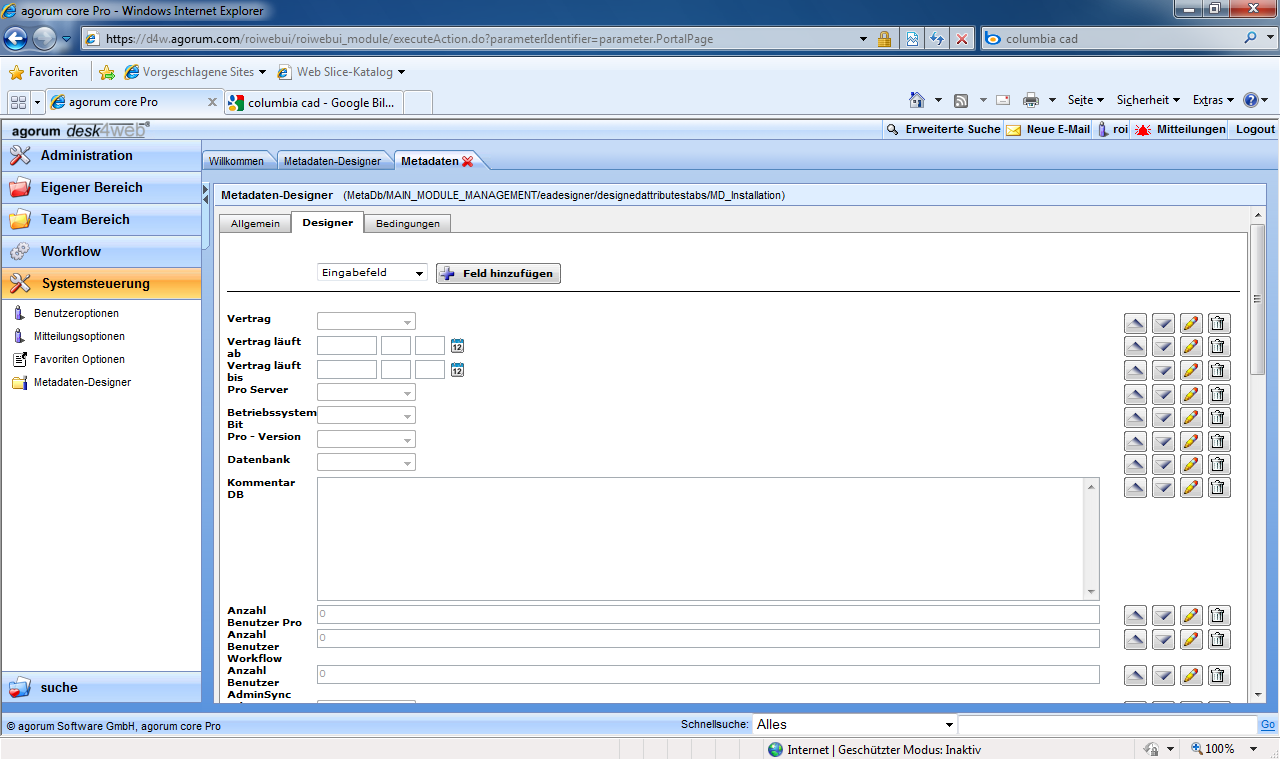
\includegraphics[width=16cm]{Bilder/agorum-core-metadatendesigner.png}
\caption{Metadaten Designer von "`agorum core"' im Web-Interface}
\label{metadatendesigner agorum}
\centering
\end{figure}

Das Einlesen und Bereitstellen von Dokumenten in "`agorum core"' funktioniert schon mit der freien Version. Jedoch kann hier nur eine Standard Suche und Ablage verwendet werden. \cite{agorum_preise}

Das automatische erkennen von Standard-Metadaten in Dateien funktioniert, jedoch auch nur mit der entsprechenden "`Pro"'-Version oder einer Zubuchung genau wie die Versionierung von Dateien.

"`agorum core"' verf\"ugt \"uber verschiedene Schnittstellen, welche von Frontends angesprochen werden k\"onnen. 

\subsection{Alfresco}
\subsection{Open Xchange}
% \subsection{anderes ECM}
\subsection{Auswertung der M\"oglichkeiten}\label{Auswertung ECM}
\textcolor{green}{\checkmark} \textcolor{red}{X} \textcolor{orange}{\checkmark X}
\newpage
\section{Implementierung des Backends auf Basis von Alfresco} \label{Implementierung Backend}
F\"ur das Backend eignet sich der Analyse aus Kapitel \ref{Technologievergleich} folgend am besten Alfresco. In den nun folgenden Abschnitten geht es um die Implementierung des Metadatenmodells aus Kapitel \ref{Erstellung eines Datenkonzepts} in Alfresco. Hierf\"ur wird zum Einen die Installation und die Arbeitsweise erl\"autert und zum Anderen wird im Hauptteil auf die Implementierung des Datenmodells in Alfresco eingegangen.

\subsection{Installation}
Die Installation von Alfresco ist denkbar einfach und unter Windows, sowie unter Linux m\"oglich. F\"ur den Download der Community Edition muss man sich mit einer g\"ultigen E-Mail-Adresse bei Alfresco anmelden\footnote{https://www.alfresco.com/de/products/community/download}. 

Die Anmeldung hat den Vorteil, dass der Nutzer zu Webinars und anderen neuen Dingen rund um Alfresco immer auf dem Laufenden ist.
Die kostenpflichtige Variante von Alfresco bietet zus\"atzliche technische Unterst\"utzung und einige Enterprise Features, welche jedoch f\"ur diese Arbeit nicht ben\"otigt werden. \cite{Wiki_Alfresco}

Nach dem Download f\"uhrt unter Linux ein Skript die Installation durch. Hierbei wird der Nutzer ausf\"uhrlich \"uber alle durgef\"uhrten Schritte informiert. Der Nutzer muss w\"ahrend der Installation ein Passwort f\"ur das Administrator-Konto angeben.\cite{Alfresco_und_Liferay}

Ist die Installation abgeschlossen und der Server gestartet, kann Alfresco im Browser lokal unter \url{http://127.0.0.1:8080/share/page/} aufgerufen werden.

War die Anmeldung erfolgreich, gelangt der Nutzer auf das "`Administrator Dashboard"', welches in Abbildung \ref{Alfresco Dashboard} im Abschnitt \ref{Alfresco} zu sehen ist.

\subsection{Metadatenmodell in Alfresco} \label{Metadatenmodell von Alfresco}
Um ein eigenes Metadatenmodell in Alfresco einf\"ugen zu k\"onnen, muss es mittels XML beschrieben werden. Unter \texttt{ALFRESCO\_HOME} wird im Folgenden das Home-Verzeichnis des Alfresco-Servers zu verstehen sein. 

In Abbildung \ref{Alfresco Content-Modell} ist das Content-Modell von Alfresco in UML dargestellt. Das Hauptelement Klasse (Class) beschreibt den Aufbau eines Content-Modells und enth\"alt Aspekte (Aspect) und Typen (Type) welche ganz oben im Diagramm zu sehen sind. \cite{Professional_Alfresco}

Klassen im Content-Modell k\"onnen ihre Eigenschaften, das hei\ss{}t ihre Aspekte und Typen, an Unterklassen vererben. In Alfresco ist nur eine einfache und keie Mehrfachvererbung zul\"assig.

Eine Klasse kann Assoziationen auf andere Klassen (Peer Association) oder Objekte (Property) enthalten. Eine Assoziation auf eine andere Klasse ist unter Alfresco jedoch nur zul\"assig, wenn schon ein Content (Instanz der Klasse) der jeweiligen Klasse existiert, andernfalls muss er vorher angelegt werden. Objekte oder auch Attribute k\"onnen aus einem Constraint oder einem einfachen Datentyp (Data Type) bestehen.

Um das Metadatenmodell, wie in Kapitel \ref{Erstellung eines Datenkonzepts} beschrieben, umsetzen zu k\"onnen, m\"ussten Datentypen auch wieder Klassen enthalten k\"onnen (Komposition). Dies ist jedoch unter keinem der beschriebenen \ac{ECM}-Tools m\"oglich. Jedoch bietet Alfresco den besten Ansatz, weshalb das Datenmodell nun noch einmal f\"ur Alfresco angepasst werden muss. Wie genau das Metadatenmodell angepasst wurde, ist im Abschnitt \ref{Ver\"andertes Datenmodell f\"ur Alfresco} genauer erl\"autert.

Unter Alfresco kann eine Klasse mehrere Typen enthalten, ein Typ kann zum Beispiel ein Bild, ein Gesetz oder \"ahnliches sein. Jeder Typ kann Attribute beinhalten, welche fest mit ihm verbunden sind. Wird eine PDF-Datei in Alfresco also zu einem "`Gesetz"' also zu ein Dokument mit dem Datentyp \texttt{Gesetz} umgewandelt, enth\"alt es unweigerlich nach der \"Anderung alle Attribute, welche direkt im Typ beschrieben und verankert sind.

Ein Aspekt kann frei definiert und zu einem beliebingen Typ hinzuf\"ugt werden. M\"ochte ein Nutzer also die Attribute von \ac{INSPIRE} hinzuf\"ugen, so reicht es, wenn er den entsprechenden Aspekt zu dem gew\"unschten Dokument hinzuf\"ugt. Die jeweiligen Datentypen m\"ussen hierbei als Aspekt definiert sein.

\begin{figure}[!ht]
\centering
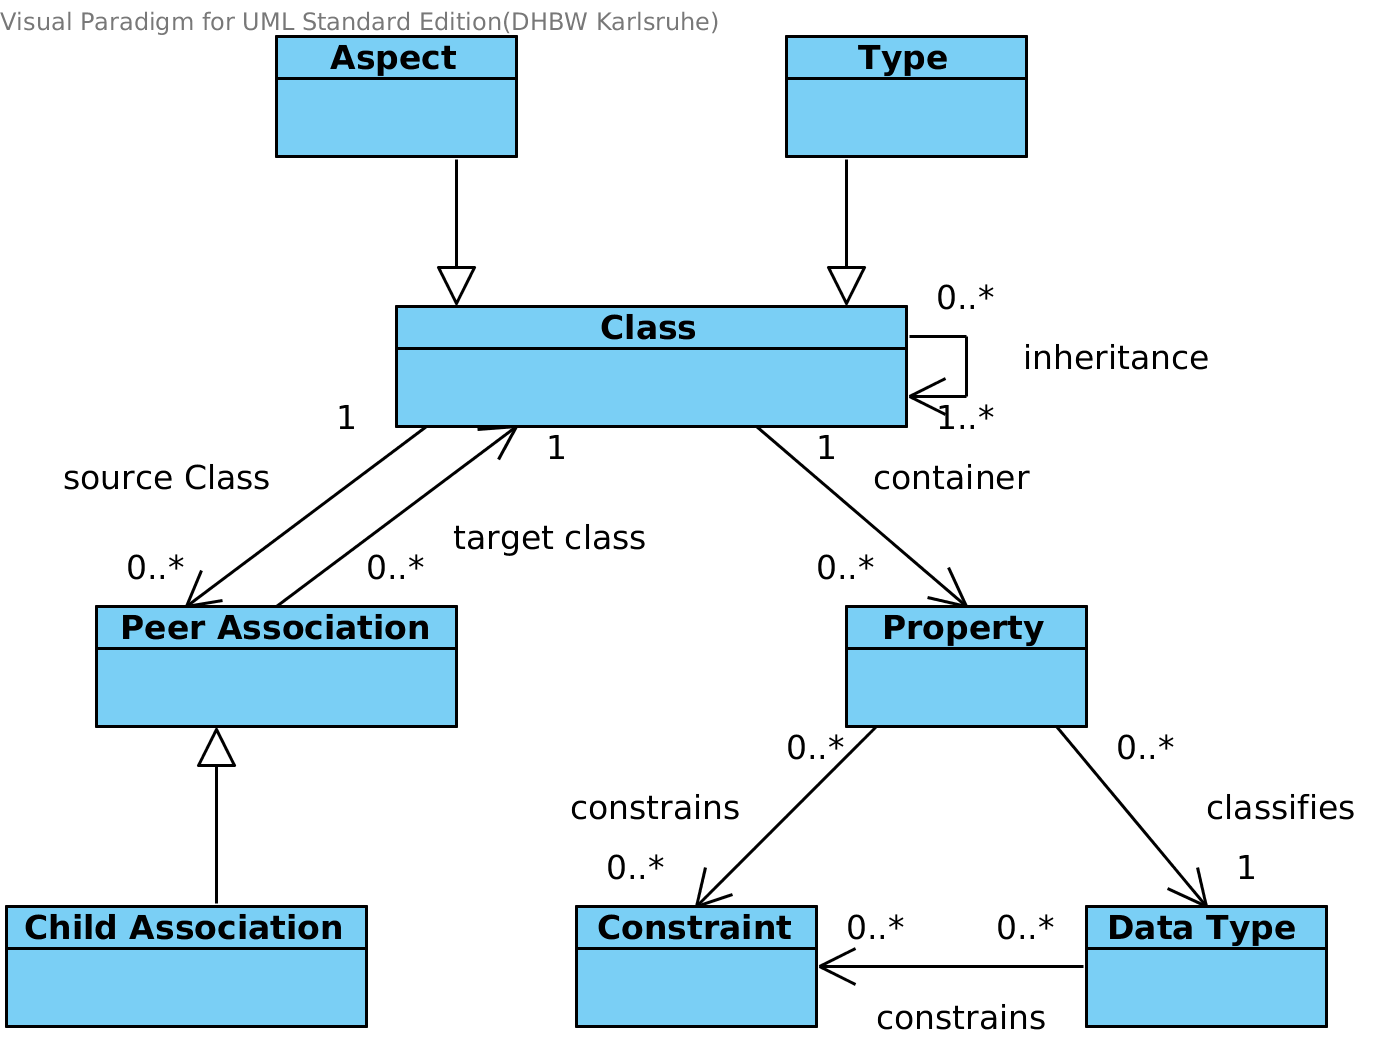
\includegraphics[width=10cm]{Bilder/Alfresco_Contentmodel.png}
\caption{Content-Modell in Alfresco}
\label{Alfresco Content-Modell}
\centering
\end{figure}

\subsection{Ver\"andertes Datenmodell f\"ur Alfresco}\label{Ver\"andertes Datenmodell f\"ur Alfresco}
Wie im Abschnitt \ref{Metadatenmodell von Alfresco} schon ausf\"uhrlich beschrieben, ist es nicht m\"oglich, die zuvor im Kapitel \ref{Erstellung eines Datenkonzepts} erstellte Metadatenstruktur umzusetzen. Daher wird nun beschrieben, wie das Datenmodell f\"ur Alfresco angepasst werden kann.

Da Alfresco den "`Dublin Core"'-Standard bereits implementiert hat, kann dieser direkt genutzt werden. Auch die Datensammlung \texttt{Datei} entf\"allt, da die entsprechenden Daten automatisch bei jeder hochgeladenen Datei von Alfresco ausgelesen und erstellt werden. 

Die im Abschnitt \ref{FADO Metadaten} gezeigten Datensammlungen werden nun zu Datentypen oder Aspekten, welche das jeweilige Dokument beschreiben. Alle farbig hinterlegten Attribute stellen Aspekte dar, die von anderen Klassen aus Alfresco \"ubernommen wurden.
Packages stellen in diesem Diagramm Klassen dar. Die UML-Klassen stellen Aspekte oder Typen dar. Worum es sich genau handelt, steht jeweils auch an den Datensammlungen. 

Alle in den folgenden Abschnitten nicht aufgef\"uhrten Datensammlungen sind direkt in den Aspekten untergebracht, da Alfresco keine Klassen oder Typen als Attribute zul\"asst.

\subsubsection{Die Datentypen}\label{Die Datentypen}
Die in den Abschnitten \ref{FADO Metadaten} bis \ref{ICT-ENSURE Metadaten} gezeigten Grunddatentypen bleiben im angepassten Modell weitestgehend identisch. Da unter Alfresco eine Datei nur von genau einem Datentyp sein kann, wurde die Datensammlung \texttt{FADO Metadaten} den anderen \ac{FADO}-Sammlungen \"ubergeordnet, wie in Abbildung \ref{Fado Datentypen f\"ur Alfresco} zu sehen ist. Der Typ \texttt{Fado Metadaten} findet sich nun in der Klasse \texttt{Fado}, welche wiederum die Oberklasse f\"ur die Typen \texttt{FADO Urteil}, \texttt{Forschungsvorhaben} und \texttt{Bibliografische Angaben} bildet.

\begin{figure}[!ht]
\centering
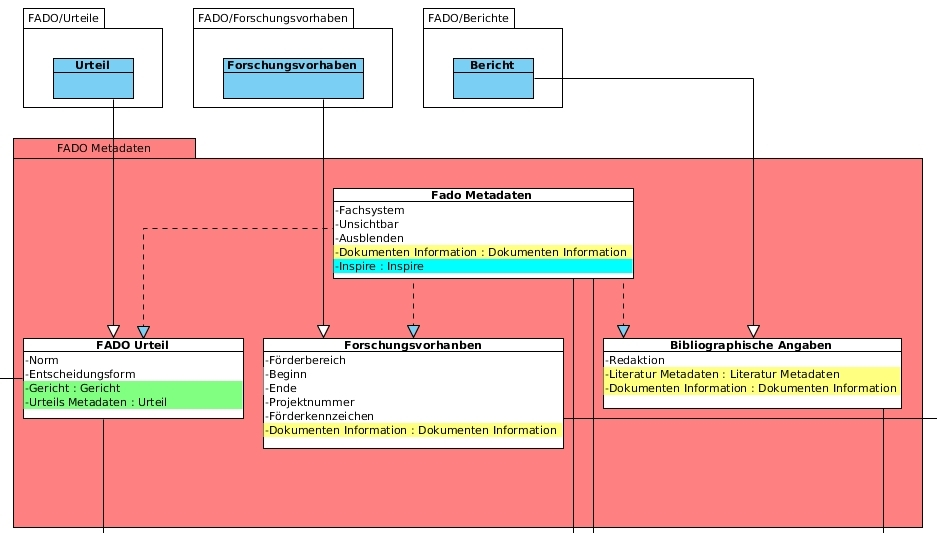
\includegraphics[width=16cm]{Bilder/AlfrescoModell/Fado-Datentypen.jpg}
\caption{FADO Datentypen f\"ur Alfresco}
\label{Fado Datentypen f\"ur Alfresco}
\centering
\end{figure}

Die Datentypen \texttt{DRS-Metadaten} und \texttt{Bildarchiv Metadaten} sind im Grunde gleich geblieben. Hier haben sich nur geringf\"ugige \"Anderungen ergeben, da die Datensammlungen wieder zusammengefasst worden sind. Die beiden Datensammlungen \texttt{Artikel Metadaten} und \texttt{Konferenz} sind zusammengefasst worden und nun im Typ \texttt{Artikel Metadaten} zu finden.
Die eben beschriebenen \"Anderungen sind in den Abbildungen \ref{Bildarchiv und ICT-ENSURE Datentypen f\"ur Alfresco} und \ref{DRS Datentyp f\"ur Alfresco} zu sehen.

\begin{figure}[!ht]
\centering
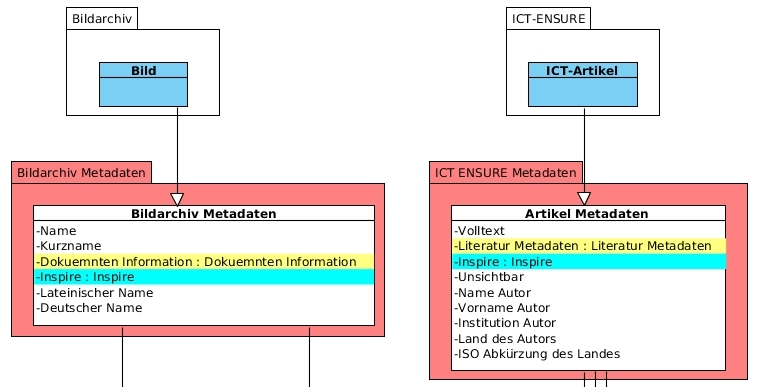
\includegraphics[width=12cm]{Bilder/AlfrescoModell/Bildarchiv-und-ICT-Datentypen.jpg}
\caption{Bildarchiv und ICT-ENSURE Datentypen f\"ur Alfresco}
\label{Bildarchiv und ICT-ENSURE Datentypen f\"ur Alfresco}
\centering
\end{figure}

Im Abschnitt \ref{Die Klasse Gerichtbarkeit} wird noch einmal genauer erw\"ahnt, warum die Attribute \texttt{Fundstelle}, \texttt{Datum Rechtsvorschriften} und \texttt{Ablage} nicht mehr existieren.

\begin{figure}[!ht]
\centering
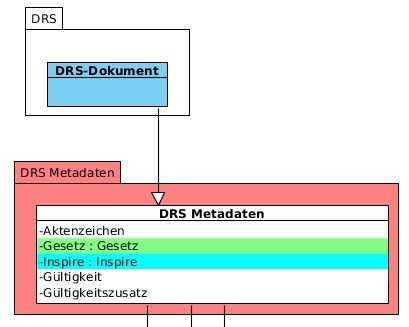
\includegraphics[width=6cm]{Bilder/AlfrescoModell/DRS-Datentypen.jpg}
\caption{DRS Datentyp f\"ur Alfresco}
\label{DRS Datentyp f\"ur Alfresco}
\centering
\end{figure}

\FloatBarrier
\subsubsection{Die Klasse Gerichtbarkeit}\label{Die Klasse Gerichtbarkeit}
Das Package \texttt{Gerichtbarkeit} beschreibt eine Klasse, welche drei Aspekte beinhaltet. Diese Aspekte sind \texttt{Gesetz}, welcher die Datensammlungen \texttt{Fundstelle}, \texttt{Datum der Rechtsvorschriften} und \texttt{Ablage} zusammengefasst, \texttt{Urtei} und \texttt{Gericht}. 

Die Datensammlung \texttt{Gericht} geht ohne Ver\"anderung in einen Aspekt \"uber und wird im Typ \texttt{FADO Urteil} verwendet. Die Sammlung \texttt{Urteil} musste etwas abge\"andert werden. Die Verweise auf das Vorgericht und das Nachgericht wurden aufgeschl\"usselt, da Alfresco bekanntlich keine Klassen als Attribute unterst\"utzt.

In Abbildung \ref{Klasse Gerichtbarkeit} ist die Klasse \texttt{Gerichtbarkeit} noch einmal dargestellt. Zu beachten ist, dass das Package hier f\"ur eine gesamte Klasse steht und die eigentlichen Klassen nur Aspekte darstellen.

\begin{figure}[!ht]
\centering
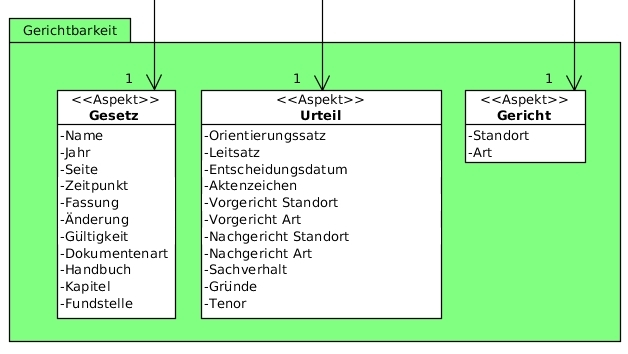
\includegraphics[width=11cm]{Bilder/AlfrescoModell/Gerichtbarkeit.jpg}
\caption{Die Klasse Gerichtbarkeit}
\label{Klasse Gerichtbarkeit}
\centering
\end{figure}

\FloatBarrier
\subsubsection{Die Klasse Standard Aspekte}\label{Die Klasse Standard Aspekte}
Das Package \texttt{Standard Aspekte}, ist wieder eine Metadaten-Klasse von Alfresco, welche den Aspekt \texttt{Inspire} enth\"alt. Durch die \"Anderungen am Datenmodell wurden die Attribute, welche sich in den verweisten Datensammlungen befunden haben, nun direkt in der Datensammlung \texttt{Inspire} untergebracht, welche nun ein Aspekt ist. 

Die Abbildung \ref{Klasse Standard Aspekte} zeigt noch einmal den Aspekt \texttt{Inspire}, welcher sich in der Klasse (dem Package) \texttt{Standard Aspekte} befindet.

\begin{figure}[!ht]
\centering
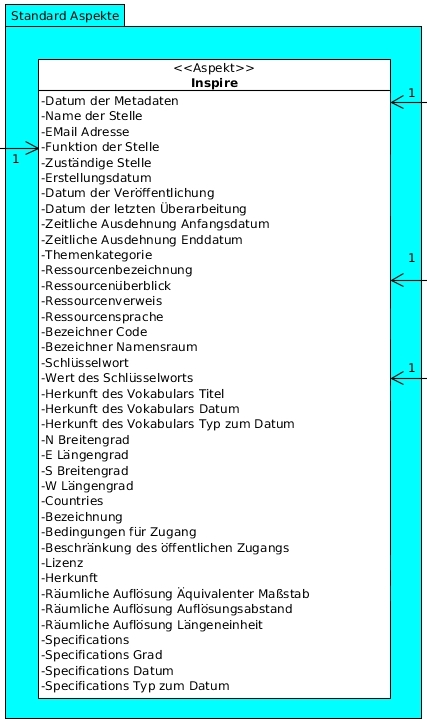
\includegraphics[width=8cm]{Bilder/AlfrescoModell/Standard-Aspekte.jpg}
\caption{Die Klasse Standard Aspekte}
\label{Klasse Standard Aspekte}
\centering
\end{figure}

\FloatBarrier
\subsubsection{Die Klasse Bibliografische Aspekte} \label{Die Klasse Bibliografische Aspekte}
In Abbildung \ref{Klasse Bibligrafische Aspekte} ist die Klasse \texttt{Bibliografische Aspekte} zu sehen, welche die beiden Aspekte \texttt{Dokumenten Information} und \texttt{Literatur Metadaten} enth\"alt.

Beim Aspekt \texttt{Dokumenten Information} ergaben sich keine \"Anderungen, au\ss{}er dass das Attribut "`Stand"' nun eigenst\"andig ist und nicht mehr auf ein Datum verweist. Der Aspekt \texttt{Literatur Metadaten} enth\"alt nun die Attribute der Datensammlungen \texttt{Kapitel} und \texttt{Publikations ID}.

\begin{figure}[!ht]
\centering
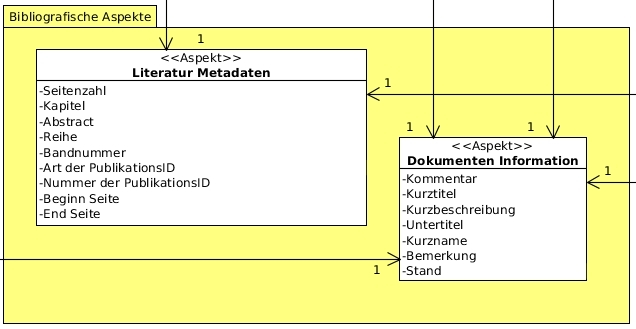
\includegraphics[width=10cm]{Bilder/AlfrescoModell/Bibliografische-Aspekte.jpg}
\caption{Die Klasse Standard Aspekte}
\label{Klasse Bibligrafische Aspekte}
\centering
\end{figure}

\FloatBarrier
\subsection{Implementierung einer Datensammlung}
Eine Datensammlung in Alfresco wird im Verzeichnis \texttt{ALFRESCO\_HOME/tomcat/shared/classes
/alfresco/extensions} abgelegt.
Wie ein Datenmodell in Alfresco implementiert wird, ist anhand der Datensammlung \texttt{Bildarchiv Metadaten} gezeigt, welche im Listing \ref{Bildarchiv-Metadaten Listing} weiter unten zu sehen ist.

Mit dem Tag "`model"' wird ein Datenmodell in Alfresco beschrieben, alle weiteren Einstellungen werden innerhalb dieses Tags vollzogen. Der Name des Modells wird durch das Prefix und die Namespace-URI gebildet.

Die Tags "`description"', "`author"' und "`version"' geben grundlegende Informationen \"uber das entsprechende Modell und wer daf\"ur verantwortlich ist.

Innerhalb des Tags "`imports"' werden Datenmodelle importiert, welche in dem Modell entsprechend verwendet werden. Grunds\"atzlich werden die Modelle \texttt{http://www.alfresco.org/model/ dictionary/1.0} und \texttt{http://www.alfresco.org/model/content/1.0} immer importiert, da sie den Grundstock eines jeden Modells bilden.

Zus\"atzlich werden die beiden Modelle \texttt{Bibliografische-Aspekte} und \texttt{Standard-Metadaten} importiert (siehe Abschnitt \ref{Die Klasse Bibliografische Aspekte} und \ref{Die Klasse Standard Aspekte}), da ihre Aspekte innerhalb des Modells verwendet werden. Hierzu sp\"ater mehr.

Der Tag "`namespaces"' definiert den Namensraum, in welchem das Datenmodell verwendet wird. Mit "`namespace"' wird der spezifische Namensraum zum einen durch eine URI, zum anderen durch ein ein Pr\"afix festgelegt. Das Pr\"afix ist eine Abk\"urzung, um nicht immer die komplette URI angeben zu m\"ussen. Die URI wiederum gibt an, wo das Datenmodell abgelegt wird, beziehungsweise zu finden ist.

"`constraints"' ist ein Tag, welcher mehrere Constraints beinhalten kann, wobei ein Constraint einen regul\"aren Ausdruck (Regex) enth\"alt und eine Zeichenfolge genauer beschreibt. Wird ein entsprechendes Constraint auf ein Textfeld angewendet, so wird beim Speichern des Dokuments von Alfresco \"uberpr\"uft, ob das jeweilige Attribut der Vorgabe des Constraints entspricht. Im Datenmodell \texttt{Bibliografische-Aspekte} gibt es keine Constraints, weshalb der entsprechende Tag leer ist.

Zus\"atzlich k\"onnen mit Constraints auch Auswahllisten realisiert werden. Hierbei werden im Constraint alle m\"oglichen Eintr\"age vorgegeben, welche sp\"ater zu Auswahl stehen sollen.

Innerhalb des Tags "`types"' k\"onnen mehrere Dokumenten-Typen spezifiziert werden. Jeder einzelne Typ ist grunds\"atzlich so aufgebaut wie der im Beispielcode in Listing \ref{Bildarchiv-Metadaten Listing} unten. Der Typ hat einen Namen, welcher mit dem Pr\"afix des jeweiligen Namensraums beginnt. 

Im Tag "`title"' wird der Standardtitel angegeben, welcher angezeigt wird, sollte keine I18N-\"Ubersetzung vorliegen. Die \"Ubersetzung wird sp\"ater noch genauer erkl\"art.

Sollte "`parent"' keine eigene Klasse sein, so steht hier standardm\"a\ss{}ig \texttt{cm:content}, welches die Standard-Oberklasse von Alfresco ist.

Unter dem Tag "`properties"' sind alle Attribute zu finden, welche der jeweilige Typ enth\"alt. Innerhalb einer "`property"' wird wiederum der Name des Attributs angegeben. Im Tag "`title"' findet sich der Standardtitel. "`type"' gibt an, von welchem Typ das Attribut ist. Eine genaue Auflistung alles Datentypen von Alfresco ist in der Dokumentation\footnote{\url{http://docs.alfresco.com/4.0/concepts/metadata-model-props.html}} zu finden. Im Tag "`constraints"' k\"onnen Verweise zu einzelnen Constraints des Datenmodells oder aber zu Constraints anderer Datenmodelle angegeben werden. 

\"Uber den Tag "`mandatory-aspects"' k\"onnen Aspekte angegeben werden, welche der Dokumententyp zwingend beinhalten muss. Im Beispiel w\"aren das die Aspekte \texttt{Inspire} und \texttt{Dokumenten-Information}. Beide Aspekte sind auch im Datenmodell in Abbildung \ref{Bildarchiv und ICT-ENSURE Datentypen f\"ur Alfresco} zu sehen.

"`aspects"' kann mehrere Aspekte der jeweiligen Klasse enthalten. Diese Aspekte k\"onnen dann innerhalb der Klasse, sowie klassen\"ubergreifend eingesetzt werden. Grunds\"atzlich sind die Beschreibungen von Aspekten genau wie die von Typen aufgebaut und beinhalten die selben Tags. Einzige Ausnahme ist der Tag "`parent"', da ein Aspekt keinen \"ubergeordneten Datentyp beinhaltet. Im Beispiel sind keine Aspekte vorhanden, da das Datenmodell dies f\"ur die Klasse \texttt{Bildarchiv Metadaten} nicht vorsieht. 

\lstinputlisting[language=xml, caption=Inhalt der Datei Bildarchiv-Metadaten.xml, label=Bildarchiv-Metadaten Listing]{Code/Bildarchiv-Metadaten.xml}

\subsubsection{Das Modell in Alfresco einbinden} \label{Das Modell in Alfresco einbinden}
Um das Datenmodell nun in Alfresco bekannt zu machen, muss eine Context-Datei erstellt werden, welche das Java-Bean beschreibt. Die Context-Datei endet auf "`-context.xml"' und muss im Ordner \texttt{ALFRESCO\_HOME/tomcat/shared/classes/alfresco/extensions} abgelegt werden.

Im Listing \ref{Bildarchiv-Metadaten-context Listing} ist die Context-Datei zu sehen, welche beschreibt wo genau die Klasse zu finden ist.
Das "`bean"' hat zum Einen eine \texttt{id} und ein \texttt{parent}. Zum Anderen ein Attribut, auf welchen Beans es bassiert, was im Attribut \texttt{depends-on} beschrieben ist. Im Beispiel sind das die beiden verwendeten Klassen welche auch importiert werden (siehe Listing \ref{Bildarchiv-Metadaten Listing}).

Unter dem Tag "`property"' wird der Speicherort unserer Modell-Datei angeben.

\lstinputlisting[language=xml, caption=Inhalt der Datei Bildarchiv-Metadaten-context.xml, label=Bildarchiv-Metadaten-context Listing]{Code/Bildarchiv-Metadaten-context.xml}

Sind beide Dateien korrekt und an der richtigen Stelle muss Alfresco neu gestartet werden um das Modell aufzunehmen.

\subsubsection{\"Ubersetzungen in Alfresco}
Um Mehrsprachigkeit in Alfresco zu realisieren verwendet das System Property-Dateien, in welchen die verschiedenen \"Ubersetzungen zu finden sind. Die Property-Dateien m\"ussen unter \texttt{ALFRESCO\_HOME/tomcat/shared/classes/alfresco/messages} abgelegt werden.

Die Dateien k\"onnen beliebig benannt werden, m\"ussen jedoch das ISO-Sprachk\"urzel am Namensende enthalten. Eine deutsche \"Ubersetzung w\"urde dann zum Beispiel in der Datei \texttt{I18N\_de\_DE.properties} und eine US-Amerikanische unter \texttt{I18N\_en\_US.properties} zu finden sein. Alfresco nutzt die �bersetzungen dann automatisch anhand der eingestellten Systemsprache.

Die Datei beinhalten pro Zeile ein Schl\"ussel-Wert-Paar, welches eine \"Ubersetzung f\"ur genau einen String darstellt.
Im Listing \ref{I18NDatei Listing} ist nur ein Ausschnitt der Datei \texttt{I18N\_de\_DE.properties} zu sehen, um das System zu verdeutlichen.

In den Property-Dateien werden Strings f\"ur Typen mit einem Schl\"ussel \texttt{type.<Namespace>\_<Typname>} bezeichnent. Aspekte werden \"ahnlich wie auch Typen bezeichnent und zwar mit \texttt{aspect.<Namespace>\_<Aspektname>}. Andere Keys, wie zum Beispiel die Keys f\"ur Hilfetexte, k\"onnen frei gew\"ahlt werden.

\lstinputlisting[caption=Ausschnitt des Inhalts der \"Ubersetzungsdatei I18N\_de\_DE.properties, label=I18NDatei Listing]{Code/I18N_de_DE.properties}

\subsection{Modell und \"Ubersetzungen in Alfresco anzeigen}
Nach dem in den vorherigen Abschnitten gezeigt wurde, wie eine Datenmodell f\"ur Alfresco erstellt und eingebunden wird, muss nun noch gekl\"art werden, wie sich \"Ubersetzungen und Datenmodell in Alfresco anzeigen lassen.

\subsubsection{Das Datenmodell anzeigen}\label{Das Datenmodell anzeigen}
Um ein Datenmodell in Alfresco mit all seinen Metadaten in der Pr\"asentation und in den Formularen anzuzeigen, reicht es nicht aus, nur das Bean zu erstellen. Zus\"atzlich muss auch angegeben werden, welche Attribute Alfresco wie darstellen soll. Die Darstellung wird in der Datei \texttt{share-config-custom.xml} beschrieben, welche sich im Verzeichnis \texttt{ALFRESCO\_HOME/tomcat/shared/classes/alfresco/web-extensions} befindet.

Da diese Config-Datei sehr lang werden kann, werden im Folgenden immer nur Ausschnitte gezeigt.

Innerhalb des Tags "`alfresco-config"' ist der im Listing \ref{Config Datenmodell} gezeigte Abschnitt zu finden, welcher jedoch hier gek\"urzt dargestellt ist. Innerhalb des Tags "`field-visibility"' m\"ussen alle Attribute aufgez\"ahlt werden die sp\"ater angezeigt werden sollen. Dies geschieht \"uber den Tag "`show"' in welchem die ID des jeweiligen Attributs angegeben werden muss. 

Die einzelnen Attribute werden, wenn sie nicht anders gegliedert sind in der Reihenfolge dargestellt wie sich hier eingetragen wurden.

Unter Tag "`field-visibility"' ist der Tag "`appearance"' zu sehen. Dieser gibt an, wie die einzelnen Attribte angezeigt werden. Als erstes werden mit dem "`set"'-Tag gruppen erzeugt, welche im Beispiel als "`bordered-panel"' angezeigt werden sollen.

Als n\"achstes werden die einzelnen Attribute mit dem Tag "`field"' noch einmal aufgelistet. Hier wird nun aufgef\"hrt, zu welcher Gruppe das Attribut geh\"ort und welchen Hilfetext es haben soll. Nat\"urlich gibt es noch weitere Einstellungsm\"oglichkeiten\footnote{\url{https://wiki.alfresco.com/wiki/Forms\_Examples\#Changing\_Set\_Appearance}}, welche im Beispiel jedoch nicht verwendet werden.

\lstinputlisting[caption=Beschreibung einer Klasse des Datemodells in der \texttt{share-config-custom.xml}, label=Config Datenmodell]{Code/Config-Datenmodell.xml}

Wie sich das setzen der Gruppierung in Alfresco auswirkt und wie es in der Dokumenten\"ubersicht genau aussieht, ist im Anhang \ref{Metadaten in der Alfrescooberfl\"ache} zu finden.

\subsubsection{Aspekte anzeigen}
Um die im Datenmodell erstellten Aspekte anzuzeigen, m\"ussen diese ebenfalls in der \texttt{share-config-custom.xml} angegeben werden.
Dies geschieht im schon vorhandenen Tag \texttt{<config evaluator="'string-compare"' condition="'DocumentLibrary"' replace="'true"'>} wie im Listing \ref{Config Aspekte} zu sehen ist. Innerhalb des Tags "`visible"' m\"ussen alle zuzuzeigenden Aspekte des Datemodells angegeben werden.

Ist diese Einstellung richtig vorgenommen wurden, k\"onnen die eigenen Aspekte nun auch zum Datentyp hinzugef\"ugt werden.

Zu beachten ist jedoch, dass nur Attribte von Aspekten angezeigt werden, die auch wie im Abschnitt \ref{Das Datenmodell anzeigen} gezeigt aufgelistet sind.

\lstinputlisting[caption=Beschreibung der Aspekte in der \texttt{share-config-custom.xml}, label=Config Aspekte]{Code/Config-Aspekte.xml}

\subsubsection{Datentyp umwandeln}
Damit die eigenen Datentypen verwendet werden k\"onnen, m\"ussen die Dokumente erst in diese Typen umgewandelt werden, denn standardm\"a\ss{}ig sind alle Dokumente vom Typ "`cm:content"'.

Damit die Typen in der Oberfl\"ache von Alfresco ge\"andert werden k\"onnen, muss dies auch in der \texttt{share-config-custom.xml} beschrieben werden. Hierf\"ur muss wie im Listing \ref{Config Typumwandlung} ein neuer "`config"'-Tag angelegt werden. Im Tag "`types"' wiederum werden die einzelnen Typen definiert, von welchen aus in andere umgewandelt werden soll. So kann im Beispiel der Typ "`cm:content"' in vier andere Typen umgewandelt werden. Dies ist m\"oglich, da diese vier Typen von "`cm:content"' erben.

Die unteren drei Datentypen erben von "`lupo-FADO:Fado-Metadaten"' und k\"onnen daher nicht direkt aus "`cm:content"' erstellt werden.

\lstinputlisting[caption=Beschreibung der Typumwandlung in der \texttt{share-config-custom.xml}, label=Config Typumwandlung]{Code/Config-Umwandlung.xml}

\subsubsection{\"Ubersetzungen einbinden}
Alfresco k\"onnen mehrere Dateien mit \"Ubersetzungen bereitgestellt werden, welche Davon verwendet wird entscheidet Alfresco automatisch Anhand der eingestellten Systemsprache. Sollte f\"ur die eingestellte Sprache keine spezielle \"Ubersetzung vorliegen so wird die Standard-Properties-Datei verwendet, welche keine Sprachk\"urzel enth\"alt in dem Falle w\"are das die Datei \texttt{I18N.properties}. 

Es muss nat\"urlich auch noch angegeben werden, wo sich die Sprachdateien befinden. Hierf\"ur muss ein Eintrag in der \texttt{custom-slingshot-application-context.xml} welche sich im Verzeichnis \texttt{ALFRESCO\_HOME/tomcat/shared/classes/alfresco/web-extensions} befindet.

Innerhalb des Tags "`list"', muss ein neuer "`value"'-Tag erstellt werden, wie es im Listing \ref{Slingshot I18N} zu sehen ist, welcher den Pfad zur Standard\"ubersetzungsdatei angibt.

\lstinputlisting[caption=Beschreibung der \texttt{custom-slingshot-application-context.xml}, label=Slingshot I18N]{Code/Slingshot-I18N.xml}

\subsection{Metadatenmodell Editor}
Eine der Anforderungen an \ac{FADO} ist, dass das Metadatenmodell einfach und ohne Programmierkenntnisse ver\"andert werden kann. Leider konnte nach einiger Recherche kein Editor gefunden werden der unter der aktuellen Version 5.0 lauff\"ahig ist. 

Aus diesem Grund sollte bei der Weiterf\"uhrung des Projekts dar\"uber nachgedacht werden eine eigene L\"osung als eigenst\"andiges Programm, oder als Alfresco-Plugin zu implementieren.

\subsection{Bulk-Import von Dateien}
Alfresco bietet die M\"oglichkeit Dateien und ihre Metadaten auch automatisiert einzulesen, dies ist vor allem hilfreich, wenn ein schon bestehendes System auf Alfresco migriert werden soll.

Der Bulk-Import geschieht \"uber die URL: \url{http://localhost:8080/alfresco/service/bulkfsimport}. Hier muss der Ordner angegeben werden, von dem die Daten eingelesen werden sollen. Zus\"atzlich muss ein Ordner innerhalb von Alfresco angegeben werden, in dem die eingelesenen Daten gespeichert werden soll. 

Es lassen sich zus\"atzlich zum Beispiel auch Stapelgr\"o\ss{}e und eine Threadanzahl einstellen, mit denen importiert wird.

Um nun auch Metadaten automatisiert einzulesen und zu speichern, m\"ussen diese in XML-Dateien abgelegt sein. Die beschreibenden XML-Dateien m\"ussen folgenden Namen tragen: \texttt{<Name der Realdatei>.<Dateiendung der Realdatei>.metadata.properties.xml}

Wird nun ein Bulk-Import gestartet, so werden aus den beschreibenden XML-Dateien die Attributwerte abgelesen.

\subsection{Verwendung von langen Textfeldern}
Bei der Implementierung des Datenmodells wurde festgestellt, dass ein Textfeld in Alfresco standardm\"a\ss{}ig nur 1.024 Zeichen lang sein kann. Problematisch wird dies vor allem bei \ac{FADO}-Dokumenten des Typs \texttt{Urteil}, denn hier k\"onnen vor allem die beiden Attribte \texttt{Tatbestand} und \texttt{Gr\"unde} die l\"ange sehr leicht \"uberschreiten. So gar L\"angen mit \"uber 27.000 Zeichen sind im aktuellen Datenbestand der \ac{LUBW} m\"oglich. Aus diesen dem genannten Grund, wurde hier etwas mehr Entwicklungsaufwand get\"atig. 

Zum Einen sollte ein so langer Text nicht als einzeiliges Textfeld dargestellt werden. Zum Anderen, muss es m\"oglich gemacht werden Texte einzugeben, welche die l\"ange von 1.024 Zeichen \"uberschreiten. Daher wurde die \texttt{share-config-custom.xml} noch einmal erweitert.

Das entsprechende Feld (im Beispiel das Attribute \texttt{Gr\"unde}) muss in seiner "`appearance"' angepasst werden, wie es im Listing \ref{appearance anpassung} zu sehen ist. Um ein mehrzeiliges Textfeld zu erzeigen, muss das "`Control-Template"' \texttt{textarea.ftl} verwendet werden. Das Template muss wie angegeben mit einer vollen Pfadangabe versehen werden, denn an dieser Stelle k\"onnten auch eigene Templates eingebunden werden.

\"Uber den Tag "`control-param"' wird mit \texttt{maxLength} die maximale L\"ange des Feldes angegeben. Im Beispiel sind es 40.000 Zeichen, was f\"ur die aktuellen \ac{FADO}-Urteile ausreicht. Wird keine maximale L\"ange angegeben, so wird das Feld standardm\"a\ss{}ig auf 1.024 Zeichen begrenzt.

Durch die Verwendung der "`Textarea"' ist es einem Nutzer m\"oglich, die Gr\"o\ss{}e des Feldes auf seine Bed\"urfnisse zu skallieren, was er mittels des Schaltf\"ache am unteren rechten Textfeldrand machen kann. \cite{Alf_Wiki_Forms}

Es w\"are auch m\"oglich, die Zeilenl\"ange fest vorzugeben, was jedoch als unpraktikabel empfunden wurde.

\lstinputlisting[caption=Appearance Anpassungen in der \texttt{share-config-custom.xml}, label=appearance anpassung]{Code/share-config_appearance.xml}

In Abbildung \ref{Textfeld Gr\"unde} ist das Textfeld nach der Bearbeitung der \texttt{share-config-custom.xml} zu sehen. Zu beobachten ist die lange Scrollleiste am rechten Rand, welche auf einen gr\"o\ss{}en Inhalt hindeutet.

\begin{figure}[!ht]
\centering
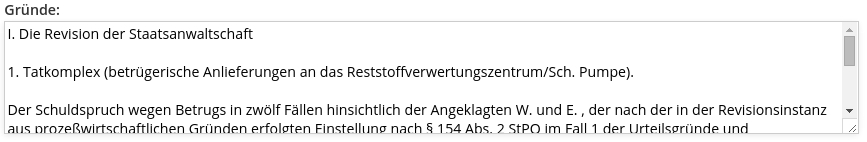
\includegraphics[width=16cm]{Bilder/Textfeld-Gruende.jpg}
\caption{Das Textfeld Gr\"unde nach der Bearbeitung}
\label{Textfeld Gr\"unde}
\centering
\end{figure}
 
\subsection{Erfahrungen aus der Alfresco-Konfiguration}
Im Internet finden sich viele Hilfestellungen und Tutorials zu Alfresco, leider nicht zu allen relevanten Themen der arbeit mit Alfresco. Deshalb sollen einige Fehlerquellen und Probleme aufgezeigt werden und wie diese gel\"ost wurden.

\subsubsection{Aufspaltung der share-config-custom.xml}
Da alle Klassen des Content-Modells mit ihren anzuzeigenden Attributen, in der \texttt{share-config-custom.xml} angegeben werden m\"ussen, w\"achst die Datei schnell an und wurde entsprechend un\"ubersichtlich.

Daher wurde die Datei aufgrspaltet und die einzelnen Bestandteile in separaten Dateien untergebracht.
Hierzu m\"ussen die neuen Dateien als Bean angegeben werden, damit Alfresco diese ber\"ucksichtigt.

Im Listing \ref{share-config Aufteilung} ist ein Ausschnitt der Datei \texttt{slingshot-application-context.xml} zu finden, welche sich im Verzeichnis \texttt{ALFRESCO\_HOME/tomcat/webapps/share/WEB-INF/classes/alfresco} befindet.

In ihr werden die einzelnen Teile der \texttt{share-config-custom.xml} mit ihren Speicherorten angegeben. Im Beispiel wurden alle Beschreibungen der Modellklassen jeweils in eigene Dateien ausgelagert.

\lstinputlisting[caption=Bean zur Aufteilung der \texttt{custom-slingshot-application-context.xml}, label=share-config Aufteilung]{Code/share-config-bean.xml}

\subsubsection{Reihenfolge der Java-Beans beachten}
Basieren die einzelnen Modellklassen aufeinander, kann es zu Fehlern kommen, wenn die einzelnen Java-Beans nicht in der richtigen Reihenfolge geladen werden. 

Importiert eine Modellklasse eine andere, so muss das in der Bean-Beschreibung auch als Abh\"angigkeit angegeben werden. Dies wurde im Abschnitt \ref{Das Modell in Alfresco einbinden} und speziell im Listing \ref{Bildarchiv-Metadaten-context Listing} schon einmal erl\"autert.

\subsection{Fehlende Funktionalit\"at im Backend}\label{Fehlende Funktionalit\"at im Backend}
Das Lastenheft im Kapitel \ref{Lastenheft} forderte eigentlich, Autoren wie Entit\"aten abzubilden, um zum Beispiel alle Werke eines Autors zu finden, ohne jedes Dokument abfragen zu m\"ussen. Leider ist dieses Vorgehen unter Alfresco nicht m\"oglich.

Alfresco ist ein \ac{ECM}-System, und verlangt f\"ur das Anlegen von Metadaten oder eines Datensatzes immer explizit ein physisches Dokument, welches entweder hochgeladenen oder direkt mit Alfresco erstellt werden muss. 

Schwierig gestaltet sich das Problem auch, da ein \ac{FADO}-Urteil keine physische Datei besitzt. Ein Urteil ist im alten System einfach als Datenbankeintrag abgebildet, ohne dass jemals eine physische Datei besteht. Bisher wurde dies im neuen System damit gel\"o\ss{}t, dass einfach eine leere Textdatei angelegt wurde, welcher dann die entsprechenden Metadaten \"ubergeben werden k\"onnen.

Die einzelnen Verweise, auf andere Fachsysteme k\"onnen durch Verweise auf Ordner (welche alle Dateien zu einem System beinhalten) nachgebildet werden. 
\newpage
\section{Implementierung des Frontends auf Basis von Liferay} \label{Implementierung Frontend}
Liferay ist ein hochperformanter Portalserver, welcher wie auch Alfresco Open Source ist. Der Nutzer hat bei Liferay die Auswahl zwischen einer kostenlosen Community Edition und einer kostenpflichtigen Enterprise Edition. Vorteil der kostenpflichtigen Enterprise Edition ist, dass hier ein Support zur Verf\"ugung steht. Au\ss{}erdem werden die kostenpflichtigen Versionen vor einer Ver\"offentlichung genauer getestet, als die Community Edition. \cite{Alfresco_und_Liferay} \cite{Wiki_Liferay}

Liferay nutzt f\"ur die Darstellung von Content sogenannte "`Portlets"'. Diese Portlets sind Anwendungen, welche Nutzern im Web zur Verf\"ungung gestellt werden.

\subsection{Alfresco als IFrame im Liferay}
In Liferay ist es m\"oglich, einen Webcontent, wie das Alfresco-Portal einer ist, als IFrame darzusellen. Der Vorteil einer solchen Umsetzung ist, dass sie schnell und einfach \"uber ein Web-Content-Portlet umgesetzt werden kann. Ein gro\ss{}er Nachteil eines solchen IFrames ist, dass er nicht ge\"andert werden kann. So ist zum Beispiel das Layout vollkommen fest vorgegeben. Auch ist es nicht sinnvoll, die komplette Alfrescooberfl\"ache innerhalb von Liferay darzustellen.

\subsection{Liferay-Repository als Frontend f\"ur Alfresco Dateien}
In der Arbeit soll untersucht werden, ob sich Liferay als Frontend f\"ur Alfresco eignet und wie ein solches ungesetzt werden kann. Da sich ein IFrame hierf\"ur absolut nicht eignet, wurde nach weiteren L\"osungen gesucht.

Liferay bietet die M\"oglichkeit, alle Dateien innerhalb der Anwendung zu verwalten und diese bei Bedarf sortiert oder gefiltert auszugeben oder anzuzeigen. Zus\"atzlich k\"onnen auch Dateien aus anderen Systemen als Repository zu Liferay hinzugef\"ugt werden. 

Das Hinzuf\"ugen eines Repositorys ist im Grunde ganz einfach, w\"are da nicht die Benutzerverwaltung. Denn um auf ein Repository von Alfresco zugreifen zu k\"onnen, muss sich der Benutzer authentifizieren. (siehe Abschnitt \ref{Benutzerverwaltung f\"ur eine Repositoryzugriff konfigurieren})

\subsubsection{Benutzerverwaltung f\"ur eine Repositoryzugriff konfigurieren}\label{Benutzerverwaltung f\"ur eine Repositoryzugriff konfigurieren}
Das im Abschnitt \ref{Alfresco als Repository im Liferay} verwendete CMIS-Repository funktioniert nur, wenn zuvor eine Authentifizierung des Nutzers stattgefunden hat. Normalerweise wird so eine Benutzerverwaltung von einem LDAP-Server oder \"uber SSO vorgenommen. 

Es reicht f\"ur die prototypische Implementierung in dieser Arbeit aber vollkommen aus, den gleichen Benutzer in beiden Systemen zu erstellen. Hierbei m\"ussen die Passw\"orter und die Benutzernamen in beiden Systemen \"ubereinstimmen.

Ist der selbe Nutzer in beiden Systemen erstellt, muss in die Liferay-Datei \texttt{portal-setup-wizard.properties} welche im Order \texttt{LIFERAY\_HOME} liegt, noch die im Listing \ref{Datei Erweiterung portal-setup-wizard.properties} zu sehende Zeile hinzugef\"ugt werden. \cite{CMIS_Repo}

\lstinputlisting[caption=Erweiterung in der Datei portal-setup-wizard.properties, label=Datei Erweiterung portal-setup-wizard.properties]{Code/portal-setup-wizard.properties}

Zus\"atzlich muss in Alfresco unter \texttt{Admin \MVRightarrow Kontrollbereich \MVRightarrow Portaleinstellungen \MVRightarrow} \\
\texttt{Authentifizierung} im Feld \texttt{Wie authentifizieren sich Nutzer?} "`Mit Benutzername"' angegeben werden.

Nach einem Neustart des Servers muss sich ab sofort mit dem Benutzernamen angemeldet werden und nicht wie zuvor mit der Mail-Adresse. \cite{CMIS_Config}

\subsubsection{Alfresco als Repository im Liferay}\label{Alfresco als Repository im Liferay}
Im Liferay kann auf der Seite "`Inhalte"' unter "`Dokumente und Medien"' ein neues Repository erzeugt werden. Es muss ein Name f\"ur das Repository gew\"ahlt werden, unter dem dieses sp\"ater zu finden ist. Als Repositorytyp muss ein \ac{CMIS}-Repository des Typs "`AtomPub"' gew\"ahlt werden. 

Die passende Repository-URL von Alfresco kann auf der Seite \url{http://127.0.0.1:8080/alfresco/} gefunden werden. Grunds\"atzlich ist es egal, ob die AtomPub Version 1.0 oder 1.1 gew\"ahlt wird. Zus\"atzlich finden sich hier auch andere Links, wie zum Beispiel ein Link f\"ur den WebDav-Zugriff auf Alfresco.

Ist die richtige URL im Feld "`AtomPub-URL"' eingetragen, muss noch die Berechtigung gew\"ahlt und anschlie\ss{}end gespeichert werden. Die Felder "`Beschreibung"' und "`Repository ID"' k\"onnen frei bleiben.

Ist alles richtig konfiguriert, sind nun alle Dateien von Alfresco in Liferay abrufbar (siehe Abbildung \ref{Repositorydarstellung in Liferay Bild} im Anhang \ref{Repositorydarstellung in Liferay}). \cite{CMIS_Repo}

Nachdem das Repository erstellt wurde, k\"onnen die Dateien aus Alfresco innerhalb von Liferay verwendet und dargestellt werden.

Sehr schnell f\"allt auf, das Liferay nur Metadaten darstellt, welche in der Datei selbst vorhanden sind. Alle anderen Metadaten, welche in Alfresco vorhanden sind werden ignoriert. In folgenden Abschnitt \ref{Untersuchungen zum Liferay-Repository} wird genauer untersucht, warum die Alfresco-Metadaten nicht dargestellt werden. \cite{Intregrate_as_Repo}

\subsubsection{Untersuchungen zum Liferay-Repository}\label{Untersuchungen zum Liferay-Repository}
Wie im Abschnitt \ref{Alfresco als Repository im Liferay} schon erkl\"art, ist Liferay nicht in der Lage, die Metadaten von Alfresco darzustellen. Im folgenden Kapitel soll nun herausgefunden werden, warum dies so ist.

Als erstes muss nat\"urlich \"uberpr\"uft werden, ob Alfresco \"uberhaupt alle vorhandenen Metadaten an anderes Systeme \"ubergibt.

\"Uber den Link im Listing \ref{Abfrage mit CMIS} k\"onnen alle Informationen zu einem Dokument (Node) abgefragt werden. Zu beachten ist, dass nat\"urlich die id bei der Verwendung ver\"andert werden muss. \cite{GetNodeInfo}

\lstinputlisting[language=html, caption=Abfrage aller Propertys eines Nodes mittels CMIS 1.1, label=Abfrage mit CMIS]{Code/getNodeInformation.html}

Beim Aufrufen des Links muss zuerst eine Authentifizierung f\"ur Alfresco angeben werden. War diese korrekt, so wird im Browser das entsprechende Element mit allen Metadaten in XML dargestellt. Dies ist zum einen die Best\"atigung, dass der \ac{CMIS}-Dienst von Alfresco ohne Probleme l\"auft, aber zum anderen auch, dass Alfresco alle vorhandenen Metadaten \"ubermittelt.

Somit liegt das Problem schon einmal nicht auf der Seite von Alfresco und es muss untersucht werden, ob die Daten im Liferay-Server richtig ankommen.

Um zu verifizieren, ob Liferay die Metadaten von Alfresco gelesen hat, muss in die Datenbank von Liferay geschaut werden.

Liferay nutzt zur internen Datenspeicherung standardm\"a\ss{}ig eine HyperSQL-Datenbank, welche vollst\"andig in Java implementiert ist und unter der BSD-Lizenz steht. Um die Datenbank auszulesen, wird ein Tool ben\"otigt, welches jedoch mit dem Liferay-Paket mitgeliefert wird. Die jar-Datei befindet ist unter \texttt{LIFERAY\_HOME/tomcat-7.0.42/lib/ext/hsql.jar}.

Nach dem Start muss als URL \url{jdbc:hsqldb:<Pfad zum Liferay-Home>/LIFERAY\_HOME/data/hsql/lportal} angegeben werden um sich mit der Datenbank zu verbinden. Vorher muss jedoch der Liferay-Server heruntergefahren werden, da dieser ein Lock auf die Datenbank h\"alt und sie somit sperrt.

Liferay kann beim einrichten des Servers aber auch mit einer anderen Datenbank wie zum Beispiel MySQL eingerichtet werden. Voraussetzung hierf\"ur ist, dass der Datendank-Server dann auf dem System vorhanden ist.

Innerhalb der Datenbank sind in der Tabelle \texttt{PUBLIC.DDMCONTENT} auch die Metadaten der Dateien abgelegt, welche \"uber das Repository eingef\"ugt wurden. In der Spalte \texttt{XML} alle Metadaten zu einem Dokument abgelegt. Hier f\"allt sofort auf, dass nicht alle Metadaten, welche Alfresco bietet, angegeben sind. Lediglich standardisierte Metadaten welche aus der Datei ausgelesen wurden, sind hier zu finden. 

Daher ist es nicht verwunderlich, dass Liferay keine weiteren Metadaten anzeigt, denn sie sind einfach nicht bekannt.

Im Folgenden muss nun gepr\"uft werden, wie die Metadaten in Liferay bekannt gemacht werden k\"onnen. Hierbei m\"ussen die Metadaten aus Alfresco ausgelesen und in Liferay gespeichert und angezeigt werden.

\subsection{Alternativen zum Liferay-Repository}
In den vorherigen Kapiteln wurde beschrieben, wie es m\"oglich ist, Alfresco-Daten in Liferay zu integrieren. Es wurde jedoch festgestellt, das Liferay standardm\"a\ss{}ig nicht in der Lage ist, die Metadaten von Alfresco-Dokumenten zu verarbeiten oder anzuzeigen. Daher wird im Folgenden nun auf Alternativen eingegangen.

Grunds\"atzlich gibt es zwei m\"ogliche Alternativen zum grundlegenden Liferay-Repository. Zum einen besteht die M\"oglichkeit ein eigenes Portlet oder Hook f\"ur Liferay zu entwickeln, zum anderen ist es m\"oglich, in den Quellcode von Liferay einzugreifen. Die M\"oglichkeit eines Eingriffs in den Quellcode ist m\"oglich, da es sich, wie schon erw\"ahnt, bei Liferay um Open Source handelt. Es w\"are somit m\"oglich, die \ac{CMIS} Schnittstelle von Liferay zu erweitern, so dass sie die von Alfresco gegebenen Metadaten verwalten kann. Nat\"urlich gibt es noch andere M\"oglichkeiten, welche in den Folgenden Abschnitten beschrieben werden.

\subsubsection{Entwicklung eines neuen Liferay-Hooks}\label{Liferay Hook}
Eine M\"oglichkeit, die fehlenden Metadaten aus Alfresco zu laden, w\"are \"uber einen Hook. Dieser sogenannte Hook ist ein Hintergrundprozess, welcher ohne grafische Schnittstelle auskommt. \cite{Liferay_in_Action}

Um \"uberhaupt eine Erweiterung f\"ur Liferay schreiben zu k\"onnen, wird die Liferay IDE\footnote{\url{http://sourceforge.net/projects/lportal/files/Liferay\%20IDE/}} ben\"otigt. Hierbei handelt es sich um eine modifizierte Eclipse-Plattform, welche einen Nutzer in die Lage versetzt, f\"ur Liferay zu entwickeln.
Aus Zeitgr\"unden kann auf die genaue Verwendung der IDE nicht eingegangen werden. 

Die Klasse des Hooks implementiert das Interface \texttt{ModelListener}, welcher auf eine \"Anderung der Klasse \texttt{RepositoryEntry} achtet.
In der implementierten Methode \texttt{onAfterCreate()} werden dann die Metadaten von Alfresco \"uber die \ac{CMIS}-Schnittstelle abgeholt und in die Liferay-Datenbank gespeichert. Die Methode wird aufgerufen, wenn ein Element aus dem Repository gelesen und in der Liferay-Datenbank angelegt wird.

F\"ur das Abrufen der Alfresco-\ac{CMIS}-Schnittstelle wurde die Apache Bibliothek "`Chemistry"'\footnote{\url{https://chemistry.apache.org/}} verwendet, welche es erm\"oglicht, \ac{CMIS}-Schnittstellen anzusprechen.

Die genaue Implementierung ist im Listing \ref{CMIS mit Chemistry} zu sehen. Es wird zuerst eine Session mit den ben\"otigten Parametern wie Username, Password und AtomPub-URL erzeugt. Dies geschieht in der selbst erstellten Methode \texttt{createCmisSession()}, welche im Anhang \ref{Methode createCmisSession} zu sehen ist.

Anschlie\ss{}end wird f\"ur das gerade erstellte Element die ID geholt und mit ihrer Hilfe das \texttt{CmisObjekt} erstellt.
Handelt es sich um einen Ordner, wird nichts weiter unternommen. Ist das Element jedoch ein Dokument, so werden alle Propertys geholt.

\"Uber einen Iterator wird durch alle Propertys durchgegangen und diese mit Hilfe der \texttt{ExpandoBridge} in die Liferay-Datenbank eingebracht.

\lstinputlisting[language=java, caption=Prototypische-Implementierung einer \ac{CMIS}-Schnittstelle mit Apache Chemistry, label=CMIS mit Chemistry]{Code/Chemistry.java}

Dieser kleine Ausflug beweist, dass es m\"oglich ist, die von Alfresco ankommenden Metadaten in Liferay zu integrieren. Somit steht auch dem Anzeigen der Metadaten auf der Oberfl\"ache nichts mehr im Wege. \cite{Chemistry_examples}

Der Aufwand, eine komplette Portierung der Metadaten umzusetzen ist relativ gering, zumal der im Prototyp vorhandene Code ohne gr\"o\ss{}ere \"Anderungen \"ubernommen werden kann. Es muss lediglich noch ein Filter eingebaut werden, um nur die gew\"unschten Metadaten in der Datenbank zu speichern.

Die Umsetzung der Anzeige und einer Suchfunktion in dem der "`Asset Publisher"' erweitert wird, sollte bei vorhandenen Daten ohne Probleme m\"oglich sein.

\subsection{Entwicklung eines neuen Liferay-Portlets}\label{Liferay Portlet}
Im Abschnitt \ref{Liferay Hook} wurde beschrieben, wie die Metadaten von Alfresco abgefragt und in der Datenbank gespeichert werden k\"onnen.

Eine andere  M\"oglichkeit, ist die Daten nicht \"uber einen Hinergrundprozess abzufragen, sondern direkt in einem Protlet. Dies hatte den Vorteil, dass eine Filterung der Metadaten nach gewissen Stichworten von Alfresco vorgenommen wird. Auch entsteht durch die Live-Abfrage keine Datenduplikation, was jedoch vermutlich die Abfragegeschindigkeit verlangsamt.
Zus\"atzlich muss f\"ur ein Portlet auch eine Oberfl\"ache implementiert werde, welche die abgefragten Daten von Alfresco anzeigt.

Ob sich daher die Implementierung eines Portlets vom Aufwand und der Abfragegeschindigkeit her lohnt kann leider nicht genau gesagt werden. Des sollte aber im Verlauf der weiteren Entwicklung als Ausblick evaluiert werden.

\subsubsection{Entwicklung von Widgets}\label{Liferay Widget}
Innerhalb der Projektgruppe werden oft kleine JavaScript-Widgets verwendet, die gewisse Informationen darstellen und auch Abfragen k\"onnen. 
Diese JavaScript-Widgets lassen sich beliebig in jede Webseite und auch in Liferay integrieren und k\"onnen dort Verwendung finden.

Es m\"usste also ein Widget geschrieben werden, welches die \ac{CMIS}-Daten von Alfresco auslie\ss{}t und diese anzeigt. Zus\"atzlich muss es auch eine Suchfunktion bieten, welche es erlaubt die Dokumente nach bestimmten Metadaten zu filtern. Der Arbeitsaufwand sollte in etwa \"ahnlich dem eines Portlets (siehe \ref{Liferay Portlet}) sein, jedoch mit dem Vorteil, dass ein solches Widget \"uberall integriert werden kann, wo JavaScript lauff\"ahig ist. 

F\"ur die Anbindung an Alfresco kann direkt die Alfresco-JavaScript-\ac{API} verwendet werden.

\subsubsection{Liferay Enterprise Edition}\label{Liferay EE}
Innerhalb der Arbeit wurde auch getestet, ob die Enterprise Edition von Liferay in der Lage ist, alle \ac{CMIS}-Daten abzufragen und zu speichern. Hierf\"ur wird die Testversion genutzt, welche zwar den vollen Funktionsumfang bietet, jedoch auf 30 Tage limitiert ist.

Es wurde kein Unterschied zum Verhalten mit der Community Edition festgestellt. Auch bietet der Store von Liferay in der Enterprise Edition keine anderen Plugins als in der Community Edition. Somit kann f\"ur die vorliegende Aufgabe auf die Enterprise Edition verzichtet werden, wenn der erweiterte Support der Enterprise Edition nicht ben\"otigt wird.

\subsubsection{Verwendung von Liferay 7}\label{Liferay 7}
In Liferay 7, welches sich zur Zeit noch in der Entwicklung befindet, werden zum einen das Dokumentmanagement von Liferay umgebaut und zum anderen wird die \ac{CMIS}-Schnittstelle erweitert. \cite{liferay7}

Es ist somit gut m\"oglich, dass Liferay sehr bald schon eigenst\"andig in der Lage ist, alle Metadaten von Alfresco anzuzeigen und zu verwalten.
Im Verlauf der Arbeit wurde eine "`Mile-Stone"'-Version installiert, um die Behauptung genauer zu pr\"ufen.

Es konnte in der Vorabversion von Liferay zwar ein Repository angelegt werden, jedoch war die Version nicht in der Lage, Dokumente zu laden. Die Logausgabe von Liferay legt nahe, dass momentan die Datenbank-Querys noch fehlerhaft sind. Daher k\"onnte die Fuktionalit\"at der neuen \ac{CMIS}-Schnittstelle nicht \"uberpr\"uft werden.

Es kann jedoch gesagt werden, dass sich in der Dateiverwaltung von Liferay einiges \"andert. Wie umfangreich diese \"Anderungen ausfallen, kann jedoch noch nicht genau gesagt werden.

\subsection{Auswertung der M\"oglichkeiten}
Es ist nicht ohne weiteres m\"oglich, die Metadaten aus Alfresco in Liferay anzuzeigen. Es wurde aber im Abschnitt \ref{Liferay Hook} gezeigt, das eine nachtr\"agliche Implementierung dieser Funktionalit\"at grundlegend m\"oglich ist. Aus zeitlichen Gr\"unden ist es aber nicht machbar gewesen, ein vollst\"andiges Beispiel zu Implementieren.

Andere Alternativen wie die Entwicklung eines Widgets, Portle oder Hooks ist grunds\"atzlich m\"oglich. Eine Implementierung ist zwar m\"oglich, jedoch aufw\"andig, weshalb dieser Ansatz nur prototypisch im Abschnitt \ref{Liferay Hook} beschrieben wurde.

Bisher ist die beste L\"osung das erweitern von Liferay \"uber einen Hook, da es f\"ur Liferay keine fertigen Plugins gibt. Eine andere M\"oglichkeit besteht darin, abzuwarten was Liferay in der Version 7 bietet. Um die Live-Abfrage von Portlets oder Widgets zu beschl\"aunigen, k\"onnten die Alfresco-Daten zum Beispiel in eine Elasticsearch\footnote{https://www.elastic.co/products/elasticsearch} Suchmaschine eingebracht und \"uber diese gesucht werden. \cite{Wiki_Elastic} \cite{elastic}

\section{Vergleich zwischen Altsystem und dem neune Prototyp}


\newpage
\section{Abk�rzungsverzeichnis}
\begin{acronym}
%   \acro{SDK}{\emph{Software Development Kits}}
%   \acro{OHA}{\emph{Open Handset Alliance}}
%   \acro{IDE}{\emph{Integrierte Entwicklungsumgebung}}
%   \acro{ADT}{\emph{Android Development Tools}}
%   \acro{DVM}{\emph{Dalvik Virtual Machine}}
%   \acro{FME}{\emph{Funkmeldeempf\"anger}}
%   \acro{JIT}{\emph{Just in Time}}
%   \acro{ART}{\emph{Android Runtime}}
%   \acro{AOT}{\emph{Ahead-of-Time-Decodierung}}
%   \acro{API}{\emph{Application Programming Interface}}
  \acro{ECM}{\emph{Enterprise Content Management}}
  \acro{DMS}{\emph{Dokumentenmanagementsystem}}
  \acro{PoC}{\emph{Proof of Concept}}
  \acro{LUBW}{\emph{Landesanstalt f\"ur Umwelt, Messungen und Naturschutz Baden-W\"urttemberg}}
  \acro{GAA}{\emph{Gewerbeaufsicht Baden-W\"urttemberg}}
  \acro{REST}{\emph{Representational State Transfer}}
  \acro{FADO}{\emph{Fachdokumente Online}}
  \acro{DRS}{\emph{Document Retrieval System}}
  \acro{INSPIRE}{\emph{Infrastructure for Spatial Information in the European Community}}
  \acro{API}{\emph{Application Programming Interface}}
  \acro{EU}{\emph{Europ\"aische Union}}
  \acro{}{\emph{}}
%  \acro{KIT}{\emph{Karlsruher Instituts f�r Technologie}}
%  \acro{GDS}{\emph{Generic Data Services}}
% %  \acro{LSDF}{\emph{Large Scale Data Facility}}
%  \acro{OPM}{\emph{Objektorientierten Programmiermodell}}
%  \acro{SMD}{\emph{Strukturelle Metadaten}}
%  \acro{JSON}{\emph{JavaScript Object Notation}}
% %  \acro{HALO}{\emph{High Altitude and Long Range Research Aircraft}}
%  \acro{IAI}{\emph{Institut f�r Angewandte Informatik}}
%  \acro{JAXB}{\emph{Java Architecture for XML Binding}}
%  \acro{UDDE}{\emph{User Data Description Editor}}
%  \acro{AMD}{\emph{Anwendermetadaten}}
%  \acro{CG}{\emph{Class Generator}}
%  \acro{IG}{\emph{Interface Generator}}
\end{acronym}
\newpage
\section{Anhang} \label{Anhang}
\subsection{Metadaten der LUBW Fachsysteme} \label{Metadaten der LUBW Fachsysteme}
In den folgenden Abschnitten sind die Metadaten und Relationen der Untersuchten Dokumente in \ac{FADO} abgebildet.
\subsubsection{Metadaten des Fachsystems FADO / Urteile}
\begin{table}[ht]
\begin{center}
\begin{tabular}{|l|l|}
\hline
\textbf{Metadaten:} & \textbf{Werte:} \\ \hline
Fachsystem & Vorgabe \\ \hline
ID & Generiert \\ \hline
Titel & Freitext \\ \hline
Tenor & Freitext \\ \hline
Kommentar & Freitext \\ \hline
Orientierungssatz & Freitext \\ \hline
Norm & Freitext \\ \hline
Leitsatz & Freitext \\ \hline
Gericht & Freitext \\ \hline
Entscheidungsform & Freitext \\ \hline
Entscheidungsdatum & Datum \\ \hline
Aktenzeichen & Freitext \\ \hline
Vorgericht & Freitext \\ \hline
Nachgericht & Freitext \\ \hline
Sachverhalt & Freitext \\ \hline
Gr�nde & Freitext \\ \hline
Unsichtbar & Bool \\ \hline
ausblenden & Bool \\ \hline
\end{tabular}
\label{Metadaten der Urteile in FADO}
\caption{Metadaten der Urteile in FADO}
\end{center}
\end{table}

\begin{table}[ht]
\begin{center}
\begin{tabular}{|l|l|}
\hline
\textbf{Relationen:} & \textbf{Werte:} \\ \hline
Thema & Vorgabe \\ \hline
geh�rt zu Fachobjekt & Vorgabe \\ \hline
hat Schlagwort & Vorgabe \\ \hline
ist vom Typ & Vorgabe \\ \hline
enthalten in Fachsystem & Vorgabe \\ \hline
wird referenziert von & Vorgabe \\ \hline
\end{tabular}
\label{Relationen der Urteile in FADO}
\caption{Relationen der Urteile in FADO}
\end{center}
\end{table}

\newpage
\subsubsection{Metadaten des Fachsystems FADO / Forschungsvorhaben}

\begin{table}[!ht]
\begin{center}
\begin{tabular}{|l|l|}
\hline
\textbf{Metadaten:} & \textbf{Werte:} \\ \hline
Fachsystem & Vorgabe \\ \hline
ID & Generiert \\ \hline
Title & Freitext \\ \hline
Kurzbeschreibung & Freitext \\ \hline
Kommentar & Freitext \\ \hline
F�rderbereich & Freitext \\ \hline
Beginn & Datum \\ \hline
Ende & Datum \\ \hline
Projektnummer & Freitext \\ \hline
F�rderkennzeichen & Freitext \\ \hline
Unsichtbar & Bool \\ \hline
ausblenden & Bool \\ \hline
\end{tabular}
\label{Metadaten der Forschungsvorhaben in FADO}
\caption{Metadaten der Forschungsvorhaben in FADO}
\end{center}
\end{table}

\begin{table}[!ht]
\begin{center}
\begin{tabular}{|l|l|}
\hline
\textbf{Relationen:} & \textbf{Werte:} \\ \hline
Thema & Vorgabe \\ \hline
geh�rt zu Fachobjekt & Vorgabe \\ \hline
hat Abschlussbericht & Vorgabe \\ \hline
hat Forschungsberichtsblatt & Vorgabe \\ \hline
hat Projektskizze & Vorgabe \\ \hline
hat Schlagwort & Vorgabe \\ \hline
hat Zwischenbericht & Vorgabe \\ \hline
wird geleitet von & Vorgabe \\ \hline
wird referenziert von & Vorgabe \\ \hline
\end{tabular}
\label{Relationen der Forschungsvorhaben in FADO}
\caption{Relationen der Forschungsvorhaben in FADO}
\end{center}
\end{table}

\newpage
\subsubsection{Metadaten des Fachsystems FADO / Berichte}

\begin{table}[!ht]
\begin{center}
\begin{tabular}{|l|l|}
\hline
\textbf{Metadaten:} & \textbf{Werte:} \\ \hline
Fachsystem & Vorgabe \\ \hline
ID & Generiert \\ \hline
Titel & Freitext \\ \hline
Kurzbeschreibung & Freitext \\ \hline
Kommentar & Freitext \\ \hline
Kurztitel & Freitext \\ \hline
Untertitel & Freitext \\ \hline
Fachthema & Freitext \\ \hline
Herausgeber & Freitext \\ \hline
Redaktion & Freitext \\ \hline
Version & Freitext \\ \hline
Stand & Datum \\ \hline
Seitenzahl & Freitext \\ \hline
Seite (von-bis) & Freitext \\ \hline
Reihe & Freitext \\ \hline
Bandnummer & Freitext \\ \hline
ISSN & Freitext \\ \hline
ISBN & Freitext \\ \hline
Preis & Freitext \\ \hline
Medium & Freitext \\ \hline
Shoprelevant & Bool \\ \hline
Shoplink & URL \\ \hline
HTML-Datei & Data \\ \hline
PDF-Datei & Data \\ \hline
Weitere Datei & Data \\ \hline
Format dieser Datei & Freitext \\ \hline
Unsichtbar & Bool \\ \hline
ausblenden & Bool \\ \hline
\end{tabular}
\label{Metadaten der Berichte in FADO}
\caption{Metadaten der Berichte in FADO}
\end{center}
\end{table}

\begin{table}[!ht]
\begin{center}
\begin{tabular}{|l|l|}
\hline
\textbf{Relationen:} & \textbf{Werte:} \\ \hline
betrift Thema & Vorgabe \\ \hline
geh�rt zu Fachobjekt & Vorgabe \\ \hline
hat Autor & Vorgabe \\ \hline
hat Schlagwort & Vorgabe \\ \hline
ist vom Typ & Vorgabe \\ \hline
enthalten in Fachsystem & Vorgabe \\ \hline
ist Abschlussbericht von & Vorgabe \\ \hline
ist Forschungsberichtsblatt von & Vorgabe \\ \hline
ist Projektskizze von & Vorgabe \\ \hline
ist Zwischenbericht von & Vorgabe \\ \hline
wird referenziert von & Vorgabe \\ \hline
\end{tabular}
\label{Relationen der Berichte in FADO}
\caption{Relationen der Berichte in FADO}
\end{center}
\end{table}

\newpage
\subsubsection{Metadaten des DRS}

\begin{table}[htbp]
\begin{center}
\begin{tabular}{|l|l|}
\hline
\textbf{Metadaten:} & \textbf{Werte:} \\ \hline
G�ltigkeit & Vorgabe \\ \hline
Titel & Freitext \\ \hline
Aktenzeichen & Freitext \\ \hline
Kurz-Titel & Vorgabe \\ \hline
Dokumentart & Vorgabe \\ \hline
Herausgeber & Vorgabe \\ \hline
Erscheinungsort & Vorgabe \\ \hline
Handbuch & Vorgabe \\ \hline
Kapitel & Vorgabe \\ \hline
Fundstelle & Vorgabe \\ \hline
Fassung & Vorgabe \\ \hline
�nderung & Vorgabe \\ \hline
Gr��e & Zahl \\ \hline
Formate & Vorgabe \\ \hline
\end{tabular}
\label{Metadaten des DRS}
\caption{Metadaten des DRS}
\end{center}
\end{table}

Zu beachten ist hier, dass die Metadaten-Tags Fassung und \"Anderung zusammengesetzte Daten enthalten, wie es in der Abbildung \ref{Suchmaske DRS} zu sehen ist.

\newpage
\subsubsection{Metadaten des Bildarchivs}

\begin{table}[htbp]
\begin{center}
\begin{tabular}{|l|l|}
\hline
\textbf{Metadaten:} & \textbf{Werte:} \\ \hline
Objektart & Freitext \\ \hline
Objektname & Freitext \\ \hline
ID & Generiert \\ \hline
URL & URL \\ \hline
Dateityp & Vorgabe \\ \hline
Name & Freitext \\ \hline
Kurzname & Freitext \\ \hline
Erstellt am & Datum \\ \hline
Autor & Freitext \\ \hline
Besitzer & Besitzer \\ \hline
Bemerkung & Freitext \\ \hline
\end{tabular}
\label{Metadaten des Bildarchivs}
\caption{Metadaten des}
\end{center}
\end{table}

\newpage
\subsection{Metadaten der ICT-ENSURE} \label{Metadaten der ICT-ENSURE}
In den folgenden Abschnitten sind die Metadaten der Dokumente der \ac{ICT-ENSURE} zu finden. Diese werden hier in UML-Form abgebildet, was auch dem eigentlichen Datenmodell hinter \ac{ICT-ENSURE} entspricht. \cite{ICT-ENSURE_Bericht}

\begin{figure}[!ht]
\centering
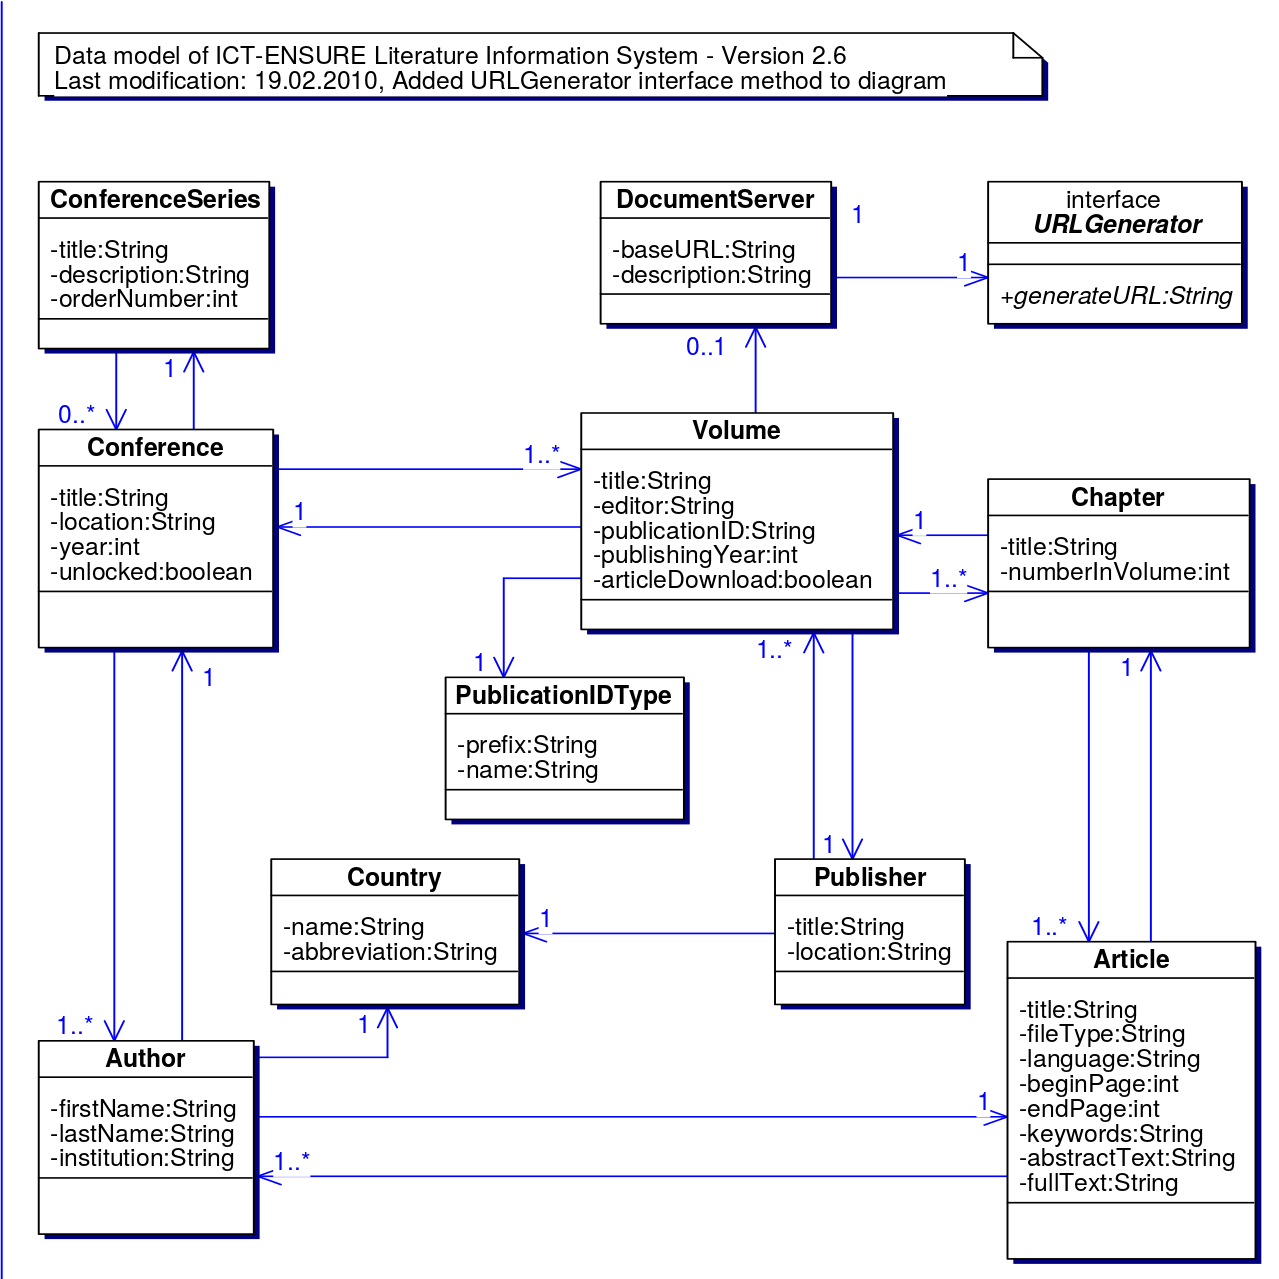
\includegraphics[width=15cm]{Bilder/Datenmodell_LitDB_V26_2010-03-11_Reduziert_fuer_Addendum.png}
\caption{Struktur von \ac{RDF}}
\label{RDF Struktur}
\centering
\end{figure}

% \subsubsection{Metadaten der Konferenzen}
% 
% \begin{table}[htbp]
% \begin{center}
% \begin{tabular}{|l|l|}
% \hline
% \textbf{Metadaten:} & \textbf{Werte:} \\ \hline
% Editor & Freitext (Mehrere Autoren) \\ \hline
% Publisher & Freitext (Bestehend aus Name und Ort) \\ \hline
% Year of Pblishing & Jahr \\ \hline
% ISBN & Freitext \\ \hline
% Conferenc & Freitext (Bestehend aus Titel, Ort, Jahr) \\ \hline
% \end{tabular}
% \label{Metadaten der Konferenzen von ICT-ENSURE}
% \caption{Metadaten der Konferenzen von ICT-ENSURE}
% \end{center}
% \end{table}
% 
% \subsubsection{Metadaten der Kapitel}
% 
% \begin{table}[htbp]
% \begin{center}
% \begin{tabular}{|l|l|}
% \hline
% \textbf{Metadaten:} & \textbf{Werte:} \\ \hline
% Editor & Freitext (Mehrere Autoren) \\ \hline
% Publisher & Freitext (Bestehend aus Name und Ort) \\ \hline
% Year of Pblishing & Jahr \\ \hline
% ISBN & Freitext \\ \hline
% Conferenc & Freitext (Bestehend aus Titel, Ort, Jahr) \\ \hline
% Editor & Freitext (Mehrere Autoren) \\ \hline
% \end{tabular}
% \label{Metadaten der Kapitel von ICT-ENSURE}
% \caption{Metadaten der Kapitel von ICT-ENSURE}
% \end{center}
% \end{table}
% 
% \subsubsection{Metadaten der Artikel}
% 
% \begin{table}[htbp]
% \begin{center}
% \begin{tabular}{|l|l|}
% \hline
% \textbf{Metadaten:} & \textbf{Werte:} \\ \hline
% Konferenz & Vorgabe \\ \hline
% Kapitel & Vorgabe \\ \hline
% Author & Freitext (ggf. Mehrere) \\ \hline
% Dateityp & Vorgabe \\ \hline
% Titel & Freitext \\ \hline
% Sprache & Freitext \\ \hline
% Beginn Seite & Zahl \\ \hline
% End Seite & Zahl \\ \hline
% Schl�sselw�rter & Freitext \\ \hline
% Abstract & Freitext \\ \hline
% Volltext & Freitext \\ \hline
% \end{tabular}
% \label{Metadaten der Vortr\"age von ICT-ENSURE}
% \caption{Metadaten der Vortr\"age von ICT-ENSURE}
% \end{center}
% \end{table}

\newpage
\listoffigures
\newpage
\listoftables
% Abk�rzungsverzeichnis
\newpage
\bibliographystyle{alpha}
% verzeichnis im DIN format
\bibliography{Quellen}
\end{document}
